\documentclass[aspectratio=169, 10pt]{beamer}
\usepackage[utf8]{inputenc}
\usepackage{amsmath, amssymb, bm, amsfonts}
\usepackage{booktabs}
\usepackage{listings}
\usepackage{graphicx}
\usepackage{tikz}
\usetikzlibrary{arrows.meta, positioning, calc, angles, quotes, shapes.geometric}

% ==============================================================================
% UNIVERSIDAD DE ANTIOQUIA (UdeA) BRANDING & THEME SETUP
% ==============================================================================
\definecolor{UdeAGreen}{HTML}{006241}
\definecolor{UdeAGold}{HTML}{D4AF37}
\definecolor{Charcoal}{HTML}{2B2B2B}
\definecolor{LightBg}{HTML}{F8F9FA}
\definecolor{DarkSlate}{RGB}{15, 23, 42}
\definecolor{AlertRed}{RGB}{220, 38, 38}
\definecolor{SpiceBlue}{RGB}{2, 132, 199}

\setbeamercolor{palette primary}{bg=UdeAGreen, fg=white}
\setbeamercolor{palette secondary}{bg=UdeAGreen, fg=white}
\setbeamercolor{structure}{fg=UdeAGreen}
\setbeamercolor{background canvas}{bg=LightBg}
\setbeamercolor{text}{fg=Charcoal}

% Block Styles
\setbeamercolor{block title}{bg=UdeAGreen, fg=white}
\setbeamercolor{block body}{bg=white, fg=Charcoal}
\setbeamercolor{block title example}{bg=UdeAGold, fg=DarkSlate}
\setbeamercolor{block body example}{bg=white, fg=Charcoal}
\setbeamercolor{block title alerted}{bg=AlertRed, fg=white}
\setbeamercolor{block body alerted}{bg=white, fg=Charcoal}

% Custom Header & Footer Setup with Lower-Right Logo
\setbeamertemplate{headline}{}
\setbeamertemplate{footline}{%
    \leavevmode%
    \hbox{%
        \begin{beamercolorbox}[wd=0.70\paperwidth,ht=2.8ex,dp=1.2ex,leftskip=.3cm]{palette primary}%
            \footnotesize Universidad de Antioquia -- Faculty of Engineering \hfill Module 2: Interplanetary Navigation
        \end{beamercolorbox}%
        \begin{beamercolorbox}[wd=0.30\paperwidth,ht=2.8ex,dp=1.2ex,rightskip=.3cm]{palette primary}%
            \hfill \insertframenumber/\inserttotalframenumber\hspace{0.25cm}%
            \raisebox{-0.15ex}{
\includegraphics[height=1.8ex,keepaspectratio]{Images/UdeA+simplificado+Negro_Smaller.png}}%
        \end{beamercolorbox}%
    }%
    \vskip0pt%
}
\setbeamertemplate{navigation symbols}{}

% Code Listings Configuration
\lstdefinestyle{gmatstyle}{
    backgroundcolor=\color{LightBg},
    basicstyle=\ttfamily\fontsize{4.6pt}{5.4pt}\selectfont\color{Charcoal},
    keywordstyle=\bfseries\color{UdeAGreen},
    commentstyle=\itshape\color{gray},
    stringstyle=\color{UdeAGold!90!black},
    frame=single,
    rulecolor=\color{UdeAGreen},
    breaklines=true,
    showstringspaces=false,
    xleftmargin=2pt,
    xrightmargin=2pt
}

\lstdefinestyle{pythoncode}{
    backgroundcolor=\color{white},
    basicstyle=\ttfamily\fontsize{4.4pt}{5.2pt}\selectfont\color{Charcoal},
    keywordstyle=\bfseries\color{UdeAGreen},
    commentstyle=\itshape\color{gray},
    stringstyle=\color{UdeAGold!90!black},
    numberstyle=\tiny\color{gray},
    numbers=left,
    numbersep=2pt,
    frame=single,
    rulecolor=\color{UdeAGreen!50},
    breaklines=true,
    showstringspaces=false,
    tabsize=2,
    xleftmargin=2pt,
    xrightmargin=2pt
}

\usetheme{Madrid}
\usefonttheme{professionalfonts}

\logo{\vspace{-0.2cm}\hfill
\includegraphics[width=1cm]{Images/UdeA+simplificado+Negro_Smaller.png}\hspace{0.1cm}}

\title[Astrodynamics Module 2]{\textbf{Module 2: 3D Interplanetary Trajectories and B-Plane Navigation}}
\subtitle{Interplanetary Flight Mechanics}
\author{\textbf{Prof. Juan Francisco Puerta Ibarra}}
%\institute{Aerospace Engineering}
\date{Semester 2026-2}
\titlegraphic{
\includegraphics[width=2.5cm,keepaspectratio]{Images/UdeA+simplificado+Negro_Smaller.png}}

\begin{document}

% ==============================================================================
% SLIDE 1: TITLE SLIDE
% ==============================================================================
\begin{frame}[plain]
    \titlepage
    \begin{center}
        \scriptsize \textcolor{DarkSlate}{\textit{Analytical Flight Mechanics, NASA SPICE Optimization, and GMAT Targeting}}
    \end{center}
\end{frame}

% ==============================================================================
% SLIDE 2: MODULE 2 ROADMAP (WITH ENLARGED TARGET DIAGRAM)
% ==============================================================================
\begin{frame}{Module 2: Architecture and Operational Roadmap}
    \begin{columns}[t]
        \begin{column}{0.68\textwidth}
            \begin{block}{From Planar Transfers to 3D Navigation}
                \fontsize{5.8pt}{6.8pt}\selectfont
                \begin{itemize}\setlength{\itemsep}{0.5pt}\setlength{\topsep}{1pt}\setlength{\parsep}{0pt}\setlength{\partopsep}{0pt}
                    \item \textbf{Week 5: 3D Patched Conics and Hyperbolic Asymptotes}
                    \begin{itemize}\setlength{\itemsep}{0.2pt}\setlength{\topsep}{0pt}\setlength{\parsep}{0pt}
                        \item Expanding 2D Lambert transfers to 3D inertial space.
                        \item Asymptote ($\alpha, \delta$) and the \textbf{Inclination Trap} ($i \ge |\delta|$).
                        \item Python 3D departure kinematics and launch azimuth solvers.
                    \end{itemize}
                    \item \textbf{Computational Mission Design: SPICE-Driven Porkchop Plots}
                    \begin{itemize}\setlength{\itemsep}{0.2pt}\setlength{\topsep}{0pt}\setlength{\parsep}{0pt}
                        \item Solving Lambert's boundary value problem via Izzo's algorithm.
                        \item Multi-planet dimensionality reduction and flyby $\Delta V$ matching.
                    \end{itemize}
                    \item \textbf{Week 6: Gravity Assists and Powered Flybys}
                    \begin{itemize}\setlength{\itemsep}{0.2pt}\setlength{\topsep}{0pt}\setlength{\parsep}{0pt}
                        \item Planetary SOI momentum transfer; turn angle $\delta_{\text{turn}}(r_p)$.
                        \item Leading vs. Trailing encounters and deep-space Oberth burns.
                    \end{itemize}
                    \item \textbf{Week 7: The B-Plane Targeting Framework}
                    \begin{itemize}\setlength{\itemsep}{0.2pt}\setlength{\topsep}{0pt}\setlength{\parsep}{0pt}
                        \item $(\hat{\mathbf{S}}, \hat{\mathbf{T}}, \hat{\mathbf{R}})$ frame and impact parameter vector $\mathbf{B}$.
                        \item Multi-variable differential correctors in NASA's GMAT.
                    \end{itemize}
                \end{itemize}
            \end{block}
        \end{column}
        
        \begin{column}{0.30\textwidth}
            \begin{alertblock}{Forensic Engineering Core}
                \scriptsize
                Planetary targeting cannot rely on point-coincidence root finders. We map state transition matrices to project miss distances onto invariant planetocentric target planes.
            \end{alertblock}
            \vspace{0.35cm}
            \centering
            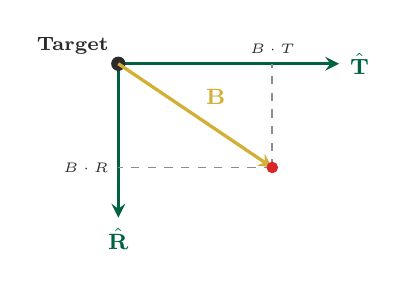
\begin{tikzpicture}[scale=0.85, >=stealth]
                % Coordinate Axes
                \draw[very thick, ->, color=UdeAGreen] (0,0) -- (3.3,0) node[right, font=\footnotesize]{$\hat{\mathbf{T}}$};
                \draw[very thick, ->, color=UdeAGreen] (0,0) -- (0,-2.3) node[below, font=\footnotesize]{$\hat{\mathbf{R}}$};
                
                % Target Center of Mass
                \filldraw[color=Charcoal] (0,0) circle (2.8pt);
                \node[above left, font=\scriptsize\bfseries, color=Charcoal] at (0,0) {Target};
                
                % Impact Parameter Vector and Components
                \draw[dashed, color=gray!90, line width=0.7pt] (2.3,-1.55) -- (2.3,0) node[above, font=\tiny, color=Charcoal]{$B\cdot T$};
                \draw[dashed, color=gray!90, line width=0.7pt] (2.3,-1.55) -- (0,-1.55) node[left, font=\tiny, color=Charcoal]{$B\cdot R$};
                \draw[very thick, ->, color=UdeAGold] (0,0) -- (2.3,-1.55) node[midway, above right, font=\footnotesize\bfseries]{$\mathbf{B}$};
                
                % Pierce Point Marker
                \filldraw[color=AlertRed] (2.3,-1.55) circle (2.2pt);
            \end{tikzpicture}
        \end{column}
    \end{columns}
\end{frame}

% ==============================================================================
% SLIDE 3: SOI LAPLACE VS HILL
% ==============================================================================
\begin{frame}{Planetary Sphere of Influence: Laplace vs. Hill Formulations}
    \begin{columns}[t]
        \begin{column}{0.51\textwidth}
            \begin{block}{Laplace Sphere of Influence ($r_{\text{SOI}}$)}
                \scriptsize
                Defines the boundary where the planetocentric 2-body approximation is more accurate than the heliocentric model:
                \vspace{-0.1cm}
                \begin{equation*}
                    \frac{a_{\text{perturb, Sun}}}{a_{\text{central, planet}}} = \frac{a_{\text{perturb, planet}}}{a_{\text{central, Sun}}} \implies r_{\text{SOI}} = d \left(\frac{\mu_p}{\mu_\odot}\right)^{2/5}
                \end{equation*}
                \vspace{-0.15cm}
                where $d$ is the planetary orbital distance from the Sun.
            \end{block}

            \vspace{-0.1cm}

            \begin{block}{Hill Sphere ($r_H$)}
                \scriptsize
                Defines the outer limit for stable closed orbits under rotating 3-body tidal forces:
                \vspace{-0.1cm}
                \begin{equation*}
                    r_H = d \left(\frac{\mu_p}{3\mu_\odot}\right)^{1/3}
                \end{equation*}
            \end{block}
        \end{column}

        \begin{column}{0.46\textwidth}
            \begin{block}{SOI Radius Comparison}
                \centering
                \scriptsize
                \setlength{\tabcolsep}{3pt}
                \begin{tabular}{lccc}
                    \toprule
                    \textbf{Body} & $\bm{d}$ \textbf{[AU]} & $\bm{r_{\text{SOI}}}$ \textbf{[km]} & $\bm{r_H}$ \textbf{[km]} \\ \midrule
                    Mercury & 0.387 & $1.12 \times 10^5$ & $2.20 \times 10^5$ \\
                    Venus   & 0.723 & $6.16 \times 10^5$ & $1.01 \times 10^6$ \\
                    Earth   & 1.000 & $9.25 \times 10^5$ & $1.50 \times 10^6$ \\
                    Moon    & 0.00257$^*$ & $6.62 \times 10^4$ & $1.29 \times 10^5$ \\
                    Jupiter & 5.204 & $4.82 \times 10^7$ & $5.31 \times 10^7$ \\ \bottomrule
                \end{tabular}
                \par\vspace{1pt}
                \tiny $^*$Moon distance relative to Earth center.
            \end{block}

            \vspace{-0.1cm}

            \begin{alertblock}{Patched Conics Boundary}
                \scriptsize
                Patched conics assumes an instantaneous switch between 2-body regimes at $r = r_{\text{SOI}}$.
            \end{alertblock}
        \end{column}
    \end{columns}
\end{frame}

% ==============================================================================
% SLIDE 4: WHY KEPLER 3RD LAW GOVERNS SOI
% ==============================================================================
\begin{frame}{Why Kepler's Third Law Governs the SOI Boundary}
    \begin{columns}[t]
        \begin{column}{0.50\textwidth}
            \begin{block}{1. Solar Tidal Gradient}
                \scriptsize
                A spacecraft at distance $r$ from a planet experiences a differential solar tidal acceleration:
                \vspace{-0.1cm}
                \begin{equation*}
                    a_{\text{tidal}} \approx \frac{\partial}{\partial d}\left(\frac{\mu_\odot}{d^2}\right) r = \frac{2\mu_\odot}{d^3} r
                \end{equation*}
            \end{block}
            \vspace{-0.1cm}
            \begin{block}{2. Kepler's 3rd Law Substitution}
                \scriptsize
                By Kepler's Third Law, the planet's orbital mean motion $n_p$ is linked to the semi-major axis $d$:
                \vspace{-0.1cm}
                \begin{equation*}
                    n_p^2 = \frac{\mu_\odot}{d^3} = \left(\frac{2\pi}{T_p}\right)^2 \implies a_{\text{tidal}} \approx 2 n_p^2 r
                \end{equation*}
            \end{block}
        \end{column}

        \begin{column}{0.47\textwidth}
            \begin{alertblock}{3. Gravitational Balance Condition}
                \scriptsize
                Equating local planetary gravity to solar tidal pull:
                \vspace{-0.1cm}
                \begin{equation*}
                    \frac{\mu_p}{r^2} \sim n_p^2 r = \frac{\mu_\odot}{d^3} r \implies r^3 \sim d^3 \left(\frac{\mu_p}{\mu_\odot}\right)
                \end{equation*}
                \vspace{-0.05cm}
                Yielding the canonical Hill radius $r_H \propto d (\mu_p / 3\mu_\odot)^{1/3}$.
            \end{alertblock}
            \vspace{-0.1cm}
            \begin{exampleblock}{Physical Consequence}
                \scriptsize
                \begin{itemize}\setlength{\itemsep}{1pt}
                    \item Fast inner planets (Mercury) endure strong solar tides ($n_p \uparrow$), shrinking their SOI.
                    \item Slow outer planets (Jupiter) have weak solar tides ($n_p \downarrow$), allowing enormous SOI volumes.
                \end{itemize}
            \end{exampleblock}
        \end{column}
    \end{columns}
\end{frame}

% ==============================================================================
% SLIDE 5: GRAVITY DETERMINATION OF MOONLESS BODIES
% ==============================================================================
\begin{frame}{Gravity Determination: Why We Must Orbit Moonless Bodies}
    \begin{columns}[t]
        \begin{column}{0.48\textwidth}
            \begin{block}{Bodies With Natural Moons}
                \scriptsize
                For bodies with moons (Earth, Mars, Jupiter), optical tracking of natural satellites yields $\mu_p$ via Kepler's 3rd Law:
                \vspace{-0.12cm}
                \begin{equation*}
                    \mu_p \approx \frac{4\pi^2 a_{\text{moon}}^3}{T_{\text{moon}}^2}
                \end{equation*}
                \vspace{-0.1cm}
                Yields high accuracy without in-situ missions.
            \end{block}

            \vspace{-0.1cm}

            \begin{alertblock}{The ``No-Moon'' Dilemma}
                \scriptsize
                \textbf{Mercury, Venus, and asteroids lack moons!}
                \begin{itemize}\setlength{\itemsep}{0pt}\setlength{\topsep}{1pt}
                    \item Pre-spaceflight mass estimates relied on weak perturbations ($\pm 1\%\text{--}5\%$ error).
                    \item Internal composition remained uncertain.
                \end{itemize}
            \end{alertblock}
        \end{column}

        \begin{column}{0.48\textwidth}
            \begin{block}{Artificial Satellite Orbit Determination}
                \scriptsize
                Placing an artificial probe in a closed orbit:
                \begin{enumerate}\setlength{\itemsep}{1pt}\setlength{\topsep}{1pt}
                    \item Radio Doppler tracking accurately measures orbit period $T_{\text{sc}}$ and semi-major axis $a_{\text{sc}}$.
                    \item Invert Kepler's Third Law:
                    \vspace{-0.12cm}
                    \begin{equation*}
                        \mu_p = \frac{4\pi^2 a_{\text{sc}}^3}{T_{\text{sc}}^2}
                    \end{equation*}
                    \vspace{-0.2cm}
                    \item Line-of-sight range-rate residuals map higher geopotential harmonics ($J_2, C_{nm}, S_{nm}$).
                \end{enumerate}
            \end{block}
        \end{column}
    \end{columns}
\end{frame}

% ==============================================================================
% SLIDE 6: WORKED EXAMPLE: MASS OF MOONLESS VENUS
% ==============================================================================
\begin{frame}{Worked Example: Measuring the Mass of Moonless Venus}
    \begin{exampleblock}{Spacecraft Orbit Benchmark (e.g., Magellan / Venus Express)}
        \scriptsize
        A science probe is placed into a circular orbit around Venus ($R_V = 6051.8\text{ km}$). DSN Doppler tracking measures an orbital altitude $h = 500.0\text{ km}$ and period $T = 5621.5\text{ s}$. \\
        Given $G = 6.67430 \times 10^{-20}\text{ km}^3/\text{kg}\cdot\text{s}^2$, $d_V = 1.0816 \times 10^8\text{ km}$, $\mu_\odot = 1.32712 \times 10^{11}\text{ km}^3/\text{s}^2$:
    \end{exampleblock}

    \vspace{-0.15cm}

    \begin{columns}[t]
        \begin{column}{0.48\textwidth}
            \scriptsize
            \textbf{Step 1: Semi-Major Axis ($a$)}
            \par\vspace{1pt}
            $a = R_V + h = 6051.8 + 500.0 = \mathbf{6551.8}\text{ km}$

            \vspace{0.08cm}
            \textbf{Step 2: Gravitational Parameter ($\mu_V$)}
            \par\vspace{1pt}
            $\mu_V = \frac{4\pi^2 a^3}{T^2} = \frac{4\pi^2 (6551.8)^3}{(5621.5)^2} = \mathbf{324858.6}\text{ km}^3/\text{s}^2$

            \vspace{0.08cm}
            \textbf{Step 3: Planetary Mass ($M_V$)}
            \par\vspace{1pt}
            $M_V = \frac{\mu_V}{G} = \frac{324858.6}{6.67430 \times 10^{-20}} = \mathbf{4.8673} \times 10^{24}\text{ kg}$
        \end{column}

        \begin{column}{0.48\textwidth}
            \scriptsize
            \textbf{Step 4: Laplace Sphere of Influence ($r_{\text{SOI}}$)}
            \begin{align*}
                r_{\text{SOI}} &= d_V \left(\frac{\mu_V}{\mu_\odot}\right)^{2/5} = (1.0816 \times 10^8)\left(\frac{324858.6}{1.32712 \times 10^{11}}\right)^{2/5} \\
                &= \mathbf{6.165} \times 10^5\text{ km} \approx \mathbf{101.9}\,R_V
            \end{align*}

            \vspace{-0.2cm}
            \begin{alertblock}{Precision Outcome}
                \scriptsize
                Direct Doppler tracking resolved $\mu_V$ to 7 significant figures, reducing mass uncertainty from $\sim 2\%$ down to $< 0.001\%$.
            \end{alertblock}
        \end{column}
    \end{columns}
\end{frame}

% ==============================================================================
% SLIDE 7: 3D PATCHED CONICS
% ==============================================================================
\begin{frame}{Week 5: 3D Patched Conics --- The Planetocentric Patch}
    \begin{columns}[t]
        \begin{column}{0.54\textwidth}
            \begin{block}{Heliocentric $\to$ Planetocentric Patching}
                \scriptsize
                \begin{itemize}\setlength{\itemsep}{1pt}
                    \item Heliocentric 3D Lambert transfer yields $\mathbf{v}_1, \mathbf{v}_2$.
                    \item \textbf{Hyperbolic Excess Velocity} vector at departure:
                    \vspace{-0.05cm}
                    \begin{equation*}
                        \mathbf{v}_{\infty,\text{dep}} = \mathbf{v}_{\text{Lambert},1} - \mathbf{v}_{\text{planet},1}
                    \end{equation*}
                    \vspace{-0.2cm}
                    \item Departure parameters: $C_3 = v_\infty^2$, $a_h = -\mu_p / v_\infty^2$, $e_h = 1 + r_p v_\infty^2 / \mu_p$.
                    \item Injection burn from parking orbit ($r_p$):
                    \vspace{-0.05cm}
                    \begin{equation*}
                        \Delta v_{\text{inj}} = \sqrt{v_\infty^2 + \frac{2\mu_p}{r_p}} - \sqrt{\frac{\mu_p}{r_p}}
                    \end{equation*}
                \end{itemize}
            \end{block}
        \end{column}

        \begin{column}{0.43\textwidth}
            \begin{block}{Asymptote Direction Unit Vector $\hat{\mathbf{S}}$}
                \scriptsize
                In Planet-Centered Inertial (PCI) frame:
                \vspace{-0.05cm}
                \begin{equation*}
                    \hat{\mathbf{S}} = \frac{\mathbf{v}_\infty}{\|\mathbf{v}_\infty\|} = \begin{bmatrix} S_x \\ S_y \\ S_z \end{bmatrix} = \begin{bmatrix} \cos\delta \cos\alpha \\ \cos\delta \sin\alpha \\ \sin\delta \end{bmatrix}
                \end{equation*}
                \vspace{-0.15cm}
                \begin{itemize}\setlength{\itemsep}{1pt}
                    \item \textbf{Declination ($\delta$):} $\delta = \arcsin(S_z) \in [-90^\circ, +90^\circ]$
                    \item \textbf{Right Ascension ($\alpha$):} $\alpha = \operatorname{atan2}(S_y, S_x)$
                \end{itemize}
            \end{block}
        \end{column}
    \end{columns}
\end{frame}

% ==============================================================================
% SLIDE 8: THE PATCHED CONIC SECTION METHOD (IMAGE OVERVIEW)
% ==============================================================================
\begin{frame}{The Patched Conic Section Method}
    \centering
    \IfFileExists{Images/IT_1.jpg}{
        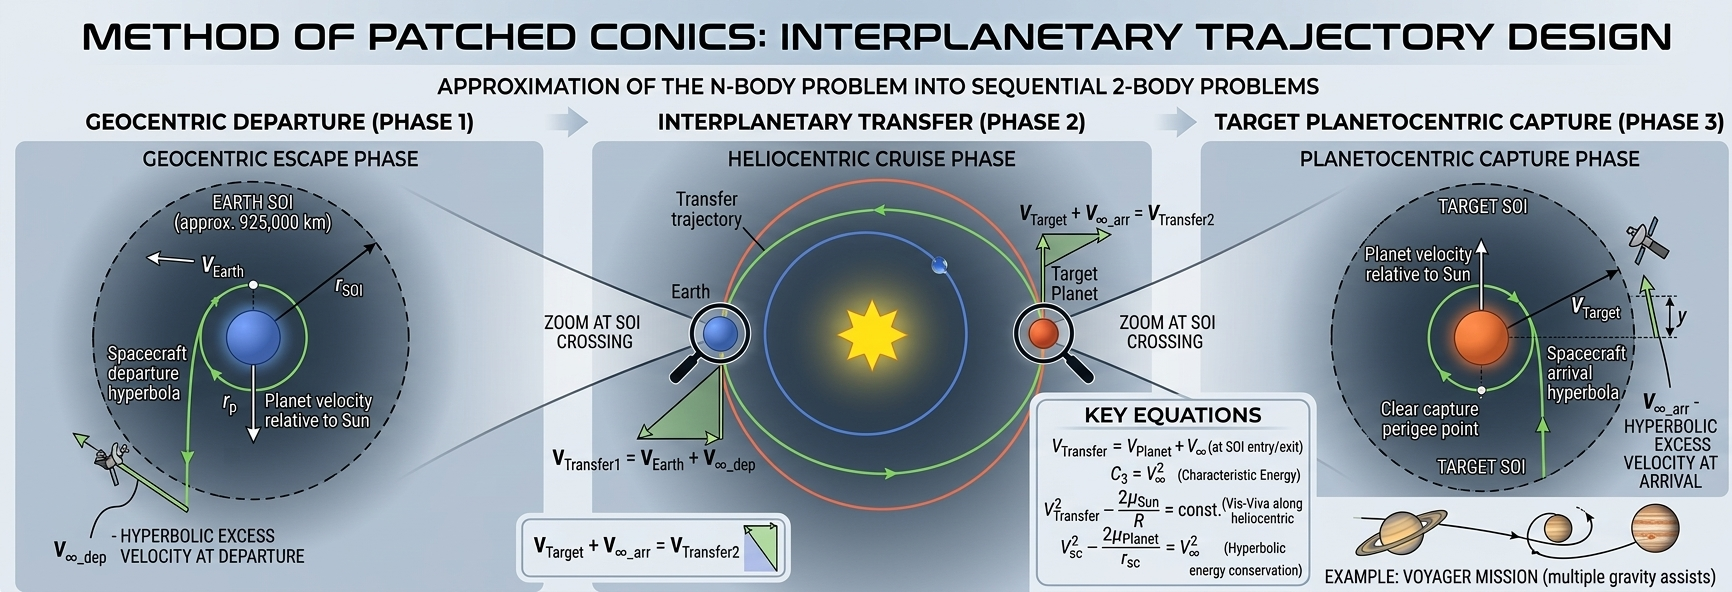
\includegraphics[width=1.0\textwidth,height=0.74\textheight,keepaspectratio]{Images/IT_1.jpg}
    }{
        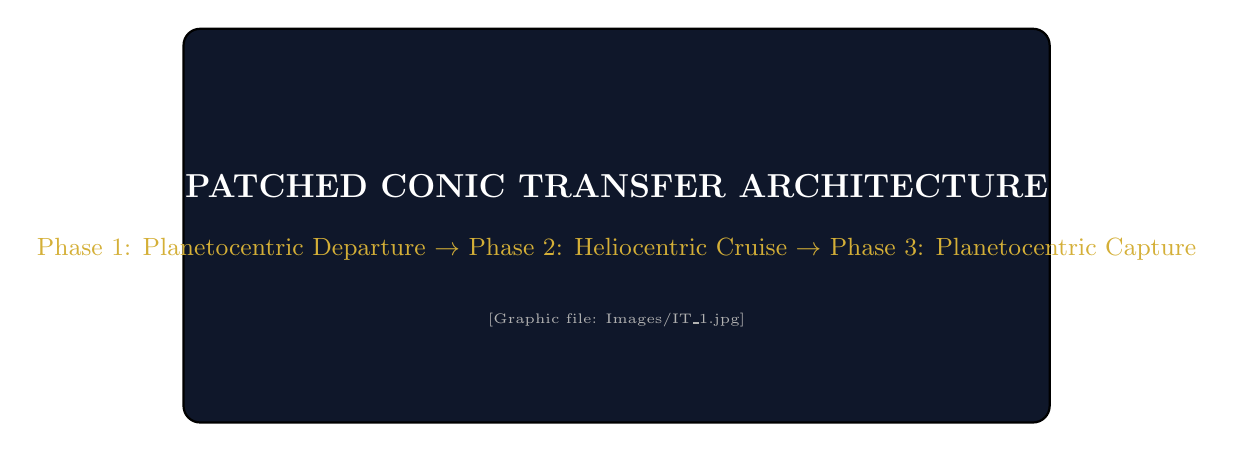
\begin{tikzpicture}
            \draw[thick, fill=DarkSlate, rounded corners=6pt] (-5.5,-2.5) rectangle (5.5,2.5);
            \node[color=white, font=\large\bfseries] at (0, 0.5) {PATCHED CONIC TRANSFER ARCHITECTURE};
            \node[color=UdeAGold, font=\small] at (0, -0.3) {Phase 1: Planetocentric Departure $\to$ Phase 2: Heliocentric Cruise $\to$ Phase 3: Planetocentric Capture};
            \node[color=gray!60, font=\tiny] at (0, -1.2) {[Graphic file: Images/IT\_1.jpg]};
        \end{tikzpicture}
    }
\end{frame}

% ==============================================================================
% SLIDE 9: METHOD OF PATCHED CONICS — 3-PHASE ARCHITECTURE
% ==============================================================================
\begin{frame}{Method of Patched Conics: The 3-Phase Architecture}
    \begin{columns}[t]
        \begin{column}{0.54\textwidth}
            \begin{block}{Approximation of the $N$-Body Problem}
                \scriptsize
                The gravitational $N$-body problem is non-integrable. The \textbf{Patched Conic Method} approximates the trajectory as three sequential 2-body Keplerian regimes:
                \begin{enumerate}\setlength{\itemsep}{2pt}\setlength{\topsep}{1pt}
                    \item \textbf{Phase 1: Planetocentric Departure ($r < r_{\text{SOI},1}$)} \\
                    Central body: Earth ($\mu_1$). Hyperbolic escape from circular parking orbit.
                    \item \textbf{Phase 2: Heliocentric Transfer ($r_{\text{SOI},1} \le R \le r_{\text{SOI},2}$)} \\
                    Central body: Sun ($\mu_\odot$). Keplerian transfer ellipse connecting departure and arrival planetary orbits.
                    \item \textbf{Phase 3: Planetocentric Arrival ($r < r_{\text{SOI},2}$)} \\
                    Central body: Target planet ($\mu_2$). Hyperbolic encounter, capture burn, or planetary flyby.
                \end{enumerate}
            \end{block}
        \end{column}

        \begin{column}{0.43\textwidth}
            \begin{block}{Patch Boundary Rule}
                \scriptsize
                \textbf{Fundamental Assumption:} At the SOI boundary ($r = r_{\text{SOI}}$), gravitational dominance switches instantaneously between the planet and the Sun:
                \vspace{-0.08cm}
                \begin{equation*}
                    \mathbf{V}_{\text{heliocentric}} = \mathbf{V}_{\text{planet}} + \mathbf{v}_{\infty}
                \end{equation*}
            \end{block}

            \vspace{-0.1cm}

            \begin{alertblock}{Energy Conservation Across Frames}
                \scriptsize
                Inside the SOI, planetocentric specific energy is conserved:
                \vspace{-0.08cm}
                \begin{equation*}
                    C_3 = v_\infty^2 = v_p^2 - \frac{2\mu_p}{r_p} = \text{const}
                \end{equation*}
            \end{alertblock}
        \end{column}
    \end{columns}
\end{frame}

% ==============================================================================
% SLIDE 10: PHASE 1 — PLANETOCENTRIC DEPARTURE & HYPERBOLIC ESCAPE
% ==============================================================================
\begin{frame}{Phase 1: Planetocentric Departure and Hyperbolic Escape}
    \begin{columns}[t]
        \begin{column}{0.50\textwidth}
            \begin{block}{Geocentric Escape Mechanics}
                \scriptsize
                \begin{enumerate}\setlength{\itemsep}{2pt}\setlength{\topsep}{1pt}
                    \item Spacecraft waits in circular parking orbit ($r_p = R_1 + h_p$) at orbital speed $v_c = \sqrt{\mu_1 / r_p}$.
                    \item Trans-Planetary Injection (TMI) burn $\Delta v_{\text{inj}}$ is executed tangentially at periapsis:
                    \vspace{-0.08cm}
                    \begin{equation*}
                        v_p = \sqrt{v_{\infty,\text{dep}}^2 + \frac{2\mu_1}{r_p}} \implies \Delta v_{\text{inj}} = v_p - v_c
                    \end{equation*}
                    \vspace{-0.15cm}
                    \item Spacecraft follows a hyperbolic escape arc, crossing Earth's SOI with excess speed $\mathbf{v}_{\infty,\text{dep}}$.
                \end{enumerate}
            \end{block}

            \vspace{-0.1cm}

            \begin{exampleblock}{Characteristic Launch Energy ($C_3$)}
                \scriptsize
                $C_3 = v_{\infty,\text{dep}}^2 = 2\mathcal{E}_h$ measures launch vehicle escape performance ($C_3 > 0$ for interplanetary escape).
            \end{exampleblock}
        \end{column}

        \begin{column}{0.47\textwidth}
            \begin{block}{Phase 1 Vector Geometry}
                \centering
                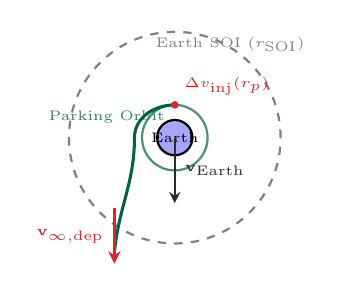
\begin{tikzpicture}[scale=0.64]
                    \draw[dashed, color=gray, line width=0.8pt] (0,0) circle (2.1cm);
                    \node[color=gray, font=\tiny] at (1.1, 1.85) {Earth SOI ($r_{\text{SOI}}$)};
                    
                    \draw[thick, color=UdeAGreen!70] (0,0) circle (0.65cm);
                    \node[color=UdeAGreen!80, font=\tiny] at (-1.35, 0.4) {Parking Orbit};
                    
                    \draw[thick, fill=blue!35] (0,0) circle (0.35cm) node[font=\tiny]{Earth};
                    \draw[thick, ->, >=stealth, color=Charcoal] (0,0) -- (0,-1.3) node[midway, right, font=\tiny]{$\mathbf{v}_{\text{Earth}}$};
                    
                    \draw[thick, color=UdeAGreen, line width=1.1pt] (0, 0.65) to[out=180, in=90] (-0.8, 0.0) to[out=-90, in=85] (-1.2, -2.3);
                    \filldraw[color=AlertRed] (0, 0.65) circle (1.8pt) node[above right, font=\tiny]{$\Delta v_{\text{inj}} (r_p)$};
                    
                    \draw[thick, ->, >=stealth, color=AlertRed, line width=1.0pt] (-1.2, -1.4) -- (-1.2, -2.5) node[midway, left, font=\tiny]{$\mathbf{v}_{\infty,\text{dep}}$};
                \end{tikzpicture}
            \end{block}
        \end{column}
    \end{columns}
\end{frame}

% ==============================================================================
% SLIDE 11: MISSION OPERATIONS — WHEN TO BURN?
% ==============================================================================
\begin{frame}{Mission Operations: When to Burn? Asymptote Alignment}
    \begin{columns}[t]
        \begin{column}{0.52\textwidth}
            \begin{block}{1. True Anomaly on the Escape Hyperbola}
                \scriptsize
                To maximize energy transfer via the \textbf{Oberth effect}, the engine burn must occur at the exact periapsis of the escape hyperbola: $\theta_{\text{burn,hyp}} = 0^\circ$.
            \end{block}

            \vspace{-0.1cm}

            \begin{block}{2. True Anomaly in the Parking Orbit}
                \scriptsize
                The heliocentric transfer dictates the required direction of asymptote $\mathbf{v}_\infty$. The asymptote angle $\beta$ from periapsis is:
                \vspace{-0.08cm}
                \begin{equation*}
                    \cos\beta = \frac{1}{e_h} = \frac{1}{1 + \frac{r_p v_\infty^2}{\mu_p}}
                \end{equation*}
                \vspace{-0.1cm}
                The spacecraft coasts in its circular parking orbit until it is positioned exactly \textbf{$\beta$ degrees away} from the target asymptote direction before firing!
            \end{block}
        \end{column}

        \begin{column}{0.45\textwidth}
            \begin{block}{Asymptote Angle Geometry ($\beta$)}
                \centering
                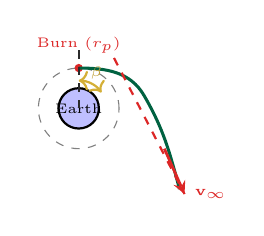
\begin{tikzpicture}[scale=0.64]
                    \draw[thick, fill=blue!25] (0,0) circle (0.40cm) node[font=\tiny]{Earth};
                    \draw[dashed, color=gray] (0,0) circle (0.80cm);
                    
                    \filldraw[color=AlertRed] (0, 0.80) circle (2pt);
                    \node[above=2pt, color=AlertRed, font=\tiny] at (0, 0.80) {Burn ($r_p$)};
                    
                    \draw[thick, color=UdeAGreen, line width=1.1pt] (0, 0.80) to[out=0, in=120] (1.3, 0.25) to[out=-60, in=105] (2.0, -1.6);
                    \draw[thick, color=Charcoal, dashed] (0,0) -- (0, 1.2);
                    
                    \draw[thick, color=AlertRed, dashed] (0.7, 1.0) -- (2.1, -1.7);
                    \draw[thick, ->, >=stealth, color=AlertRed, line width=1pt] (1.7, -0.8) -- (2.1, -1.7) node[right, font=\tiny]{$\mathbf{v}_\infty$};
                    
                    \draw[<->, color=UdeAGold, line width=0.8pt] (0, 0.55) arc (90:35:0.55);
                    \node[color=UdeAGold!90!black, font=\tiny\bfseries] at (0.35, 0.70) {$\beta$};
                \end{tikzpicture}
            \end{block}

            \vspace{-0.15cm}

            \begin{alertblock}{Operational Rule}
                \scriptsize
                Ignition must occur at true anomaly $\theta_p = \theta_\infty - \beta$. An anomaly error of $1^\circ$ causes a multi-thousand-kilometer miss at arrival.
            \end{alertblock}
        \end{column}
    \end{columns}
\end{frame}

% ==============================================================================
% SLIDE 12: THE OBERTH EFFECT & ENERGY MULTIPLICATION
% ==============================================================================
\begin{frame}{The Oberth Effect: Energy Multiplication at High Velocity}
    \begin{columns}[t]
        \begin{column}{0.50\textwidth}
            \begin{block}{Kinetic Energy Lever Arm}
                \scriptsize
                Kinetic energy scales quadratically ($E_k = \frac{1}{2} m v^2$). Applying an impulsive burn $\Delta v$ at speed $v$:
                \vspace{-0.08cm}
                \begin{equation*}
                    \Delta \mathcal{E}_k = \frac{1}{2}(v + \Delta v)^2 - \frac{1}{2}v^2 = v \Delta v + \frac{1}{2}(\Delta v)^2 \approx v \Delta v
                \end{equation*}
                \vspace{-0.05cm}
                Current speed $v$ acts as a \textbf{linear multiplier} on energy gain for the same propellant mass.
            \end{block}

            \vspace{-0.08cm}

            \begin{block}{The Deep-Well Departure Advantage}
                \scriptsize
                Compare burning $\Delta v$ at periapsis ($v_p$) vs.\ in deep cruise ($v_\infty$):
                \begin{itemize}\setlength{\itemsep}{1pt}
                    \item \textbf{Deep Space Burn:} $\Delta C_3 = 2 v_\infty \Delta v + (\Delta v)^2$
                    \item \textbf{Periapsis Burn ($r_p$):} $\Delta C_3 = 2 v_p \Delta v + (\Delta v)^2$
                \end{itemize}
                Because $v_p = \sqrt{v_\infty^2 + 2\mu/r_p} \gg v_\infty$, burning deep in Earth's gravity well dramatically magnifies excess energy $C_3$.
            \end{block}
        \end{column}

        \begin{column}{0.47\textwidth}
            \begin{block}{Exhaust Energy Transfer Mechanism}
                \centering
                \vspace{0.05cm}
                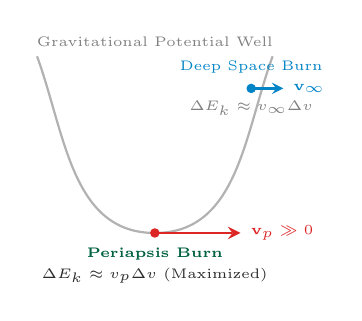
\begin{tikzpicture}[scale=0.68]
                    \draw[thick, color=gray!60] (-2.2, 1.8) to[out=-70, in=180] (0, -1.5) to[out=0, in=-110] (2.2, 1.8);
                    \node[above, font=\tiny, color=gray] at (0, 1.8) {Gravitational Potential Well};

                    \filldraw[color=AlertRed] (0, -1.5) circle (2.2pt);
                    \draw[thick, ->, >=stealth, color=AlertRed, line width=1pt] (0, -1.5) -- (1.6, -1.5) node[right, font=\tiny]{$\mathbf{v}_p \gg 0$};
                    \node[below=2pt, font=\tiny\bfseries, color=UdeAGreen] at (0, -1.5) {Periapsis Burn};
                    \node[below=9pt, font=\tiny, color=Charcoal] at (0, -1.5) {$\Delta E_k \approx v_p \Delta v$ (Maximized)};

                    \filldraw[color=SpiceBlue] (1.8, 1.2) circle (2.2pt);
                    \draw[thick, ->, >=stealth, color=SpiceBlue, line width=0.8pt] (1.8, 1.2) -- (2.4, 1.2) node[right, font=\tiny]{$\mathbf{v}_\infty$};
                    \node[above=2pt, font=\tiny, color=SpiceBlue] at (1.8, 1.2) {Deep Space Burn};
                    \node[below=1pt, font=\tiny, color=gray] at (1.8, 1.2) {$\Delta E_k \approx v_\infty \Delta v$};
                \end{tikzpicture}
            \end{block}

            \vspace{-0.1cm}

            \begin{alertblock}{Propellant Energy Accounting}
                \scriptsize
                Chemical energy is fixed. When burned at high velocity, the exhaust is left behind with near-zero inertial kinetic energy, transferring nearly all fuel energy into the spacecraft.
            \end{alertblock}
        \end{column}
    \end{columns}
\end{frame}

% ==============================================================================
% SLIDE 13: WHAT IS C3?
% ==============================================================================
\begin{frame}{What is $C_3$? Characteristic Energy Defined}
    \begin{columns}[t]
        \begin{column}{0.50\textwidth}
            \begin{block}{Definition of Characteristic Energy ($C_3$)}
                \scriptsize
                In interplanetary mission design, launch energy is quantified by the \textbf{Characteristic Energy ($C_3$)}:
                \vspace{-0.08cm}
                \begin{equation*}
                    C_3 = v_\infty^2 = 2 \mathcal{E}_h \quad [\text{km}^2/\text{s}^2]
                \end{equation*}
            \end{block}

            \begin{block}{Physical Meaning}
                \scriptsize
                $C_3$ measures specific energy to escape Earth and reach target:
                \begin{itemize}\setlength{\itemsep}{1.2pt}
                    \item $\mathbf{C_3 = 0}$: Parabolic escape ($v_\infty = 0$), matching Earth's solar orbit.
                    \item $\mathbf{C_3 > 0}$: Hyperbolic excess $v_\infty$ to reach outer/inner planets.
                \end{itemize}
            \end{block}
        \end{column}

        \begin{column}{0.47\textwidth}
            \begin{block}{Why Use $C_3$ Instead of $\Delta V$?}
                \scriptsize
                \begin{enumerate}\setlength{\itemsep}{2pt}
                    \item \textbf{Isolates the Interplanetary Problem:} \\
                    $\Delta V$ depends on parking altitude $r_p$. In contrast, $C_3$ is an absolute energy metric independent of parking orbit geometry!
                    \item \textbf{Direct Launch Vehicle Sizing:} \\
                    Launch providers publish payload curves: $\text{Mass} = f(C_3)$. A mission requirement of $C_3 = 15\text{ km}^2/\text{s}^2$ directly determines payload capacity for Falcon Heavy, Vulcan, or SLS.
                \end{enumerate}
            \end{block}
        \end{column}
    \end{columns}
\end{frame}

% ==============================================================================
% SLIDE 14: ANALYTICAL EXAMPLE: EARTH TO VENUS
% ==============================================================================
\begin{frame}{Analytical Example: Earth to Venus (Inner Trajectory)}
    \begin{exampleblock}{Mission Scenario}
        \scriptsize
        Departure from Earth circular parking orbit ($h_p = 300\text{ km}$) to Venus via heliocentric transfer. \\
        Earth: $R_\oplus = 149.6 \times 10^6\text{ km}$, $V_\oplus = 29.78\text{ km/s}$. \quad Venus: $R_V = 108.2 \times 10^6\text{ km}$.
    \end{exampleblock}

    \vspace{-0.15cm}

    \begin{columns}[t]
        \begin{column}{0.48\textwidth}
            \scriptsize
            \textbf{Step 1: Transfer Semi-Major Axis ($a_{\text{tx}}$)}
            \par\vspace{1pt}
            $a_{\text{tx}} = \frac{R_\oplus + R_V}{2} = \frac{149.6 + 108.2}{2} \times 10^6 = \mathbf{128.9} \times 10^6\text{ km}$

            \vspace{0.06cm}
            \textbf{Step 2: Departure Speed ($V_{\text{tx},1}$)}
            \par\vspace{1pt}
            $V_{\text{tx},1} = \sqrt{\mu_\odot \left(\frac{2}{R_\oplus} - \frac{1}{a_{\text{tx}}}\right)} = \mathbf{27.29}\text{ km/s}$

            \vspace{0.06cm}
            \textbf{Step 3: Hyperbolic Excess ($v_\infty$) and $C_3$}
            \par\vspace{1pt}
            $v_{\infty,\text{dep}} = |V_{\text{tx},1} - V_\oplus| = |27.29 - 29.78| = \mathbf{2.49}\text{ km/s}$
            \par\vspace{1pt}
            $C_3 = v_\infty^2 = (2.49)^2 = \mathbf{6.20}\text{ km}^2/\text{s}^2$
        \end{column}

        \begin{column}{0.48\textwidth}
            \scriptsize
            \textbf{Step 4: Trans-Venus Injection Burn ($\Delta v_{\text{inj}}$)}
            \par\vspace{1pt}
            $r_p = R_\oplus + h_p = 6378 + 300 = 6678\text{ km}$
            \par\vspace{1pt}
            $v_c = \sqrt{\mu_\oplus / r_p} = 7.73\text{ km/s}, \quad v_p = \sqrt{v_\infty^2 + 2\mu_\oplus / r_p} = 11.21\text{ km/s}$
            \par\vspace{1pt}
            $\Delta v_{\text{inj}} = v_p - v_c = 11.21 - 7.73 = \mathbf{3.48}\text{ km/s}$

            \vspace{0.06cm}
            \textbf{Step 5: Time of Flight ($TOF$)}
            \par\vspace{1pt}
            $TOF = \pi \sqrt{\frac{a_{\text{tx}}^3}{\mu_\odot}} = 1.262 \times 10^7\text{ s} \approx \mathbf{146.1}\text{ days}$
        \end{column}
    \end{columns}
\end{frame}

% ==============================================================================
% SLIDE 15: THE INCLINATION TRAP
% ==============================================================================
\begin{frame}{The Launch Geometry Boundary: The "Inclination Trap"}
    \begin{columns}[t]
        \begin{column}{0.50\textwidth}
            \begin{alertblock}{The Mathematical Constraint: $i \ge |\delta|$}
                \scriptsize
                \begin{itemize}\setlength{\itemsep}{1.5pt}
                    \item Parking orbit reaches maximum latitude $\phi_{\max} = i$.
                    \item For departure burn $\Delta \mathbf{v}_{\text{inj}}$ to be executed \textbf{in-plane} (zero out-of-plane penalty):
                    \vspace{-0.05cm}
                    \begin{equation*}
                        \sin i = \cos \delta \sin(\beta_{\text{inertial}}) \implies i \ge |\delta|
                    \end{equation*}
                    \vspace{-0.15cm}
                    \item If $i < |\delta|$ (\textbf{The Inclination Trap}), no coplanar injection exists!
                    \item Forces costly non-coplanar wedge burn:
                    \vspace{-0.05cm}
                    \begin{equation*}
                        \Delta v_{\text{penalty}} \approx 2 v_{\text{park}} \sin\left(\frac{\Delta \psi}{2}\right)
                    \end{equation*}
                \end{itemize}
            \end{alertblock}
        \end{column}

        \begin{column}{0.47\textwidth}
            \begin{block}{Launch Azimuth $\beta_{\text{launch}}$}
                \scriptsize
                From launch latitude $\phi_L$ into inclination $i$:
                \vspace{-0.05cm}
                \begin{equation*}
                    \cos \beta = \frac{\cos i}{\cos \phi_L}
                \end{equation*}
                \centering
                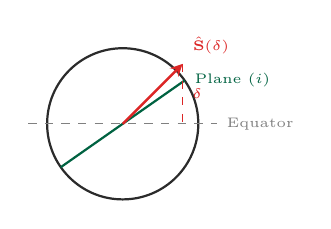
\begin{tikzpicture}[scale=0.80]
                    \draw[thick, color=Charcoal] (0,0) circle (1.2cm);
                    \draw[dashed, color=gray] (-1.5,0) -- (1.5,0) node[right, font=\tiny]{Equator};
                    \draw[thick, color=UdeAGreen, rotate=35] (-1.2,0) -- (1.2,0) node[right, font=\tiny]{Plane ($i$)};
                    \draw[thick, ->, >=stealth, color=AlertRed, line width=0.9pt] (0,0) -- (0.95,0.95) node[above right, font=\tiny]{$\hat{\mathbf{S}} (\delta)$};
                    \draw[dashed, color=AlertRed] (0.95,0.95) -- (0.95,0) node[midway, right, font=\tiny]{$\delta$};
                \end{tikzpicture}
            \end{block}
        \end{column}
    \end{columns}
\end{frame}

% ==============================================================================
% SLIDE 16: WORKED EXAMPLE 1 (EARTH TO MARS)
% ==============================================================================
\begin{frame}{Worked Example 1: Earth-to-Mars Departure Geometry}
    \begin{exampleblock}{Analytical Trajectory Benchmark}
        \scriptsize
        Lambert: $\mathbf{v}_{\text{Lambert}} = [32.45, 12.10, 4.85]\text{ km/s}$, Earth: $\mathbf{v}_{\oplus} = [29.78, 0.00, 0.00]\text{ km/s}$. \\
        $h_p = 250\text{ km}$ ($R_{\oplus} = 6378\text{ km}, \mu_{\oplus} = 398600.44\text{ km}^3/\text{s}^2$). Launch site: $\phi_L = 28.5^\circ$.
    \end{exampleblock}

    \vspace{-0.15cm}

    \begin{columns}[t]
        \begin{column}{0.48\textwidth}
            \scriptsize
            \textbf{Step 1: Hyperbolic Excess Vector ($\mathbf{v}_\infty$)}
            \begin{align*}
                \mathbf{v}_\infty &= \mathbf{v}_{\text{Lambert}} - \mathbf{v}_{\oplus} = [2.67, 12.10, 4.85]\text{ km/s} \\
                v_\infty &= \sqrt{2.67^2 + 12.10^2 + 4.85^2} = \mathbf{13.31}\text{ km/s} \\
                C_3 &= v_\infty^2 = \mathbf{177.27}\text{ km}^2/\text{s}^2
            \end{align*}
            \vspace{-0.15cm}
            \textbf{Step 2: Asymptote Declination and RA}
            \begin{equation*}
                \delta = \arcsin(4.85/13.31) = +\mathbf{21.37}^\circ, \quad \alpha = \mathbf{77.56}^\circ
            \end{equation*}
        \end{column}

        \begin{column}{0.48\textwidth}
            \scriptsize
            \textbf{Step 3: Check Inclination Trap}
            \begin{equation*}
                i_{\text{park}} = 28.5^\circ \ge |\delta| = 21.37^\circ \quad \textcolor{UdeAGreen}{\textbf{[PASS]}}
            \end{equation*}
            \textbf{Step 4: Trans-Mars Injection $\Delta v_{\text{TMI}}$}
            \begin{align*}
                r_p &= 6378 + 250 = 6628\text{ km} \\
                v_{\text{park}} &= \sqrt{\mu/r_p} = 7.755\text{ km/s} \\
                v_{\text{periapsis}} &= \sqrt{v_\infty^2 + 2\mu/r_p} = 17.247\text{ km/s} \\
                \Delta v_{\text{TMI}} &= 17.247 - 7.755 = \mathbf{9.492}\text{ km/s}
            \end{align*}
        \end{column}
    \end{columns}
\end{frame}

% ==============================================================================
% SLIDE 17: PYTHON SCRIPT: DEPARTURE & INCLINATION TRAP SOLVER
% ==============================================================================
\begin{frame}[fragile]{Python Implementation: 3D Departure and Inclination Trap Solver}
    \begin{columns}[t]
        \begin{column}{0.48\textwidth}
            \begin{block}{Mathematical Routine Architecture}
                \scriptsize
                The Python function solves 3D asymptotic kinematics:
                \begin{enumerate}\setlength{\itemsep}{1.5pt}
                    \item Subtracts Earth's velocity to yield $\mathbf{v}_\infty$.
                    \item Computes characteristic energy $C_3 = \|\mathbf{v}_\infty\|^2$.
                    \item Determines asymptote angles: $\delta = \arcsin(S_z)$, $\alpha = \operatorname{atan2}(S_y, S_x)$.
                    \item Evaluates the \textbf{Inclination Trap} ($i_{\text{park}} \ge |\delta|$).
                    \item Calculates coplanar launch azimuths $\beta_{\text{launch}} = \pm \arccos(\cos i / \cos \phi_L)$.
                    \item Computes $\Delta v_{\text{TMI}}$ from circular parking orbit $r_p$.
                \end{enumerate}
            \end{block}
        \end{column}

        \begin{column}{0.50\textwidth}
\begin{lstlisting}[style=pythoncode]
import numpy as np

def solve_3d_departure(v_lambert, v_planet, phi_L_deg, hp_km):
    mu_earth = 398600.44; R_earth = 6378.14
    v_inf = np.array(v_lambert) - np.array(v_planet)
    v_inf_mag = np.linalg.norm(v_inf)
    C3 = v_inf_mag**2
    
    # Asymptote Declination and Right Ascension
    S = v_inf / v_inf_mag
    delta = np.arcsin(S[2])
    alpha = np.arctan2(S[1], S[0])
    
    # Check Inclination Trap from direct launch (i = phi_L)
    i_park = np.radians(phi_L_deg)
    trap_violation = abs(delta) > i_park
    
    # Sizing Trans-Mars Injection
    rp = R_earth + hp_km
    v_park = np.sqrt(mu_earth / rp)
    v_peri = np.sqrt(v_inf_mag**2 + 2 * mu_earth / rp)
    dv_inj = v_peri - v_park
    
    # Launch Azimuth
    cos_beta = np.cos(i_park) / np.cos(np.radians(phi_L_deg))
    beta_deg = np.degrees(np.arccos(np.clip(cos_beta, -1, 1)))
    
    return {"C3": C3, "delta_deg": np.degrees(delta), 
            "alpha_deg": np.degrees(alpha), "trap": trap_violation,
            "dv_inj": dv_inj, "beta_launch": beta_deg}
\end{lstlisting}
        \end{column}
    \end{columns}
\end{frame}

% ==============================================================================
% SLIDE 18: THE REALITY OF INTERPLANETARY FLIGHT
% ==============================================================================
\begin{frame}{The Reality of Interplanetary Flight: Beyond Hohmann}
    \begin{columns}[t]
        \begin{column}{0.50\textwidth}
            \begin{block}{Why Coplanar Hohmann Fails in Practice}
                \scriptsize
                Standard textbook Hohmann transfers assume planets move in perfect, coplanar circles. In reality:
                \begin{itemize}\setlength{\itemsep}{1.2pt}
                    \item Planetary orbits are \textbf{eccentric} ($e_{\text{Mars}} = 0.0934$, $e_{\text{Mercury}} = 0.2056$).
                    \item Planetary orbits are \textbf{mutually inclined} ($i_{\text{Mars}} = 1.85^\circ$, $i_{\text{Mercury}} = 7.00^\circ$).
                    \item A pure $180^\circ$ Hohmann transfer rarely exists!
                    \item The required launch energy ($C_3$) and arrival speed ($v_{\infty,\text{arr}}$) change drastically with calendar dates.
                \end{itemize}
            \end{block}
        \end{column}

        \begin{column}{0.47\textwidth}
            \begin{alertblock}{The Numerical Solution: Lambert Sweeps}
                \scriptsize
                Instead of idealized conics, computers solve \textbf{Lambert's Problem} across thousands of calendar date pairs:
                \vspace{-0.08cm}
                \begin{equation*}
                    (\mathbf{r}_1(t_{\text{dep}}), \, \mathbf{r}_2(t_{\text{arr}}), \, \Delta t) \xrightarrow{\text{Lambert}} (\mathbf{V}_1, \, \mathbf{V}_2)
                \end{equation*}
                \vspace{-0.01cm}
                Mapping the resulting $C_3$ values over a 2D departure/arrival grid reveals the trajectory landscape: \textbf{The Porkchop Plot}!
            \end{alertblock}
        \end{column}
    \end{columns}
\end{frame}

% ==============================================================================
% SLIDE 19: THE PORKCHOP PLOT
% ==============================================================================
\begin{frame}{Mapping the Energy Landscape: The Porkchop Plot}
    \begin{columns}[t]
        \begin{column}{0.48\textwidth}
            \begin{block}{Anatomy of a Porkchop Plot}
                \scriptsize
                \begin{itemize}\setlength{\itemsep}{1.2pt}
                    \item \textbf{X-Axis:} Departure Date ($t_{\text{dep}}$ from Earth).
                    \item \textbf{Y-Axis:} Arrival Date ($t_{\text{arr}}$ at target planet).
                    \item \textbf{Contour Lines:} Constant Characteristic Energy ($C_3$).
                    \item \textbf{Dashed Lines:} Time of Flight ($TOF = t_{\text{arr}} - t_{\text{dep}}$).
                    \item \textbf{The ``Valleys'' (Dark Blue Centers):} Optimal launch windows requiring minimum $C_3$ / minimum propellant!
                \end{itemize}
            \end{block}
        \end{column}

        \begin{column}{0.49\textwidth}
            \begin{block}{Porkchop Contour Schematic}
                \centering
                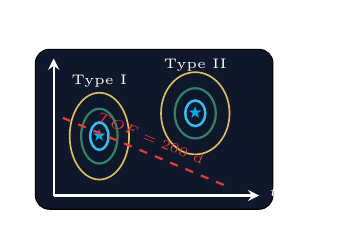
\begin{tikzpicture}[scale=0.58]
                    \draw[fill=DarkSlate, rounded corners=5pt] (-2.6,-1.7) rectangle (2.6, 1.8);
                    
                    \draw[->, >=stealth, color=white, line width=0.8pt] (-2.2,-1.4) -- (2.3,-1.4) node[right, font=\tiny]{$t_{\text{dep}}$};
                    \draw[->, >=stealth, color=white, line width=0.8pt] (-2.2,-1.4) -- (-2.2,1.6) node[above, font=\tiny]{$t_{\text{arr}}$};
                    
                    \draw[color=UdeAGold!80, line width=0.6pt] (-1.2,-0.1) ellipse (0.65cm and 0.95cm);
                    \draw[color=UdeAGreen!80, line width=0.8pt] (-1.2,-0.1) ellipse (0.40cm and 0.60cm);
                    \draw[color=cyan!80, line width=0.9pt] (-1.2,-0.1) ellipse (0.20cm and 0.30cm);
                    \node[color=cyan, font=\tiny] at (-1.2,-0.1) {$\bigstar$};
                    \node[color=white, font=\tiny] at (-1.2, 1.1) {Type I};
                    
                    \draw[color=UdeAGold!80, line width=0.6pt] (0.9, 0.4) ellipse (0.75cm and 0.90cm);
                    \draw[color=UdeAGreen!80, line width=0.8pt] (0.9, 0.4) ellipse (0.45cm and 0.55cm);
                    \draw[color=cyan!80, line width=0.9pt] (0.9, 0.4) ellipse (0.22cm and 0.28cm);
                    \node[color=cyan, font=\tiny] at (0.9, 0.4) {$\bigstar$};
                    \node[color=white, font=\tiny] at (0.9, 1.45) {Type II};
                    
                    \draw[dashed, color=AlertRed!90, line width=0.8pt] (-2.0, 0.3) -- (1.6, -1.2) node[midway, above, sloped, font=\tiny]{$TOF = 200\text{ d}$};
                \end{tikzpicture}
            \end{block}
        \end{column}
    \end{columns}
\end{frame}

% ==============================================================================
% SLIDE 20: PORKCHOP PLOT ALGORITHM
% ==============================================================================
\begin{frame}{Launch Window Determination: The Porkchop Grid Algorithm}
    \begin{columns}[t]
        \begin{column}{0.50\textwidth}
            \begin{block}{Steps 1 to 3: The Lambert Sweep Loop}
                \fontsize{6.0pt}{7.0pt}\selectfont
                \begin{enumerate}\setlength{\itemsep}{1pt}\setlength{\topsep}{1pt}
                    \item \textbf{Define Constraints:} Select bodies, calendar spans ($t_{\text{dep}}, t_{\text{arr}}$), and launcher $C_3$ limits.
                    \item \textbf{Initialize 2D Grid:} Set calendar step size ($\Delta t = 2\text{ days}$) across departure and arrival axes.
                    \item \textbf{Execute Lambert Sweep (For each point):}
                    \begin{itemize}\setlength{\itemsep}{0.5pt}
                        \item Query ephemerides $\mathbf{r}_1(t_{\text{dep}}), \mathbf{r}_2(t_{\text{arr}})$ from SPICE kernels.
                        \item Solve Lambert BVP for $TOF = t_{\text{arr}} - t_{\text{dep}}$ to obtain $\mathbf{V}_1, \mathbf{V}_2$.
                        \item Departure excess: $\mathbf{v}_\infty = \mathbf{V}_1 - \mathbf{V}_{\text{planet},1}$.
                        \item Store grid energy: $C_3 = \|\mathbf{v}_\infty\|^2$.
                    \end{itemize}
                \end{enumerate}
            \end{block}
        \end{column}

        \begin{column}{0.47\textwidth}
            \begin{block}{Steps 4 and 5: Window Selection}
                \fontsize{6.0pt}{7.0pt}\selectfont
                \begin{enumerate}\setcounter{enumi}{3}\setlength{\itemsep}{1.2pt}\setlength{\topsep}{1pt}
                    \item \textbf{Generate Contour Map:} Plot 2D isopower contours of $C_3$, filtering unfeasible domains ($C_3 > C_{3,\max}$).
                    \item \textbf{Identify Opportunity Valleys:}
                    \begin{itemize}\setlength{\itemsep}{0.8pt}
                        \item Locate local energy minima (valleys) in the contours.
                        \item Trade $C_3$ against flight time and arrival speed $v_{\infty,\text{arr}}$.
                        \item Select between \textbf{Type I} ($\Delta\nu < 180^\circ$) and \textbf{Type II} ($\Delta\nu > 180^\circ$) transfer geometries.
                    \end{itemize}
                \end{enumerate}
            \end{block}
        \end{column}
    \end{columns}
\end{frame}

% ==============================================================================
% SLIDE 21: TYPE I VS TYPE II TRAJECTORIES
% ==============================================================================
\begin{frame}{Trajectory Topologies: Type I vs. Type II Transfers}
    \begin{columns}[t]
        \begin{column}{0.48\textwidth}
            \begin{block}{Type I Trajectories ($\Delta\nu < 180^\circ$)}
                \fontsize{6.0pt}{7.0pt}\selectfont
                \begin{itemize}\setlength{\itemsep}{1.2pt}
                    \item True anomaly change is less than half an orbit ($\Delta\nu < 180^\circ$).
                    \item \textbf{Shorter Time of Flight:} Spacecraft reaches target before aphelion ($\sim 200\text{ days}$ for Mars).
                    \item Often incurs slightly higher $C_3$ or higher arrival velocity $v_{\infty,\text{arr}}$.
                \end{itemize}
            \end{block}
            \vspace{-0.1cm}
            \begin{block}{Type II Trajectories ($\Delta\nu > 180^\circ$)}
                \fontsize{6.0pt}{7.0pt}\selectfont
                \begin{itemize}\setlength{\itemsep}{1.2pt}
                    \item True anomaly change exceeds half an orbit ($\Delta\nu > 180^\circ$).
                    \item \textbf{Longer Time of Flight:} Spacecraft passes aphelion before intercepting the planet ($\sim 250\text{--}300\text{ days}$).
                    \item Often yields lower $C_3$ launch energy, maximizing payload capacity!
                \end{itemize}
            \end{block}
        \end{column}

        \begin{column}{0.48\textwidth}
            \begin{exampleblock}{Real Mission Case: Mars 2020 (Perseverance)}
                \scriptsize
                Mission planners used porkchop plot analysis to select a \textbf{Type II trajectory}:
                \begin{itemize}\setlength{\itemsep}{1pt}
                    \item Launched: July 30, 2020.
                    \item Landed at Jezero Crater: February 18, 2021.
                    \item Trading slightly longer cruise time for lower $C_3$ allowed launching the massive $1025\text{ kg}$ rover and Ingenuity helicopter on an Atlas V 541!
                \end{itemize}
            \end{exampleblock}
        \end{column}
    \end{columns}
\end{frame}

% ==============================================================================
% SLIDE 22: COMPUTATIONAL ENGINE: SOLVING LAMBERT'S PROBLEM
% ==============================================================================
\begin{frame}{Computational Engine: Solving Lambert's BVP via Izzo's Algorithm}
    \begin{columns}[t]
        \begin{column}{0.54\textwidth}
            \begin{block}{Keplerian Boundary Value Formulation}
                \scriptsize
                Determine the transfer orbit connecting planetary positions $\mathbf{r}_1$ and $\mathbf{r}_2$ in gravitational parameter $\mu$ over time of flight $\Delta t = t_2 - t_1$:
                \vspace{-0.08cm}
                \begin{equation}
                    \Delta t = f(a, \|\mathbf{r}_1\| + \|\mathbf{r}_2\|, c)
                \end{equation}
                \vspace{-0.15cm}
                where $c = \|\mathbf{r}_2 - \mathbf{r}_1\|$ is the geometric chord.
            \end{block}
            \vspace{-0.1cm}
            \begin{block}{Izzo's Algorithm in \texttt{poliastro.iod.izzo}}
                \scriptsize
                \begin{itemize}\setlength{\itemsep}{1pt}
                    \item Parameterizes transfer geometry using transformed chord variables $(x, y)$.
                    \item Solves for semi-major axis $a$ using rapid Householder iterations.
                    \item Computes departure velocity $\mathbf{v}_1$ and arrival velocity $\mathbf{v}_2$.
                    \item Multi-revolution indexing: selects the 0-revolution direct solution (\texttt{sol[0]}).
                \end{itemize}
            \end{block}
        \end{column}

        \begin{column}{0.44\textwidth}
            \begin{block}{Lambert Transfer Geometry}
                \centering
                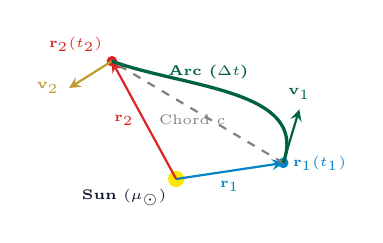
\begin{tikzpicture}[scale=0.68]
                    \filldraw[color=yellow!90!orange] (0,0) circle (4pt) node[below left, font=\tiny, color=DarkSlate]{\textbf{Sun} ($\mu_\odot$)};
                    
                    \coordinate (R1) at (2.0, 0.3);
                    \draw[thick, ->, >=stealth, color=SpiceBlue] (0,0) -- (R1) node[midway, below, font=\tiny] {$\mathbf{r}_1$};
                    \filldraw[color=SpiceBlue] (R1) circle (2.5pt) node[right, font=\tiny] {$\mathbf{r}_1(t_1)$};
                    \draw[thick, ->, >=stealth, color=UdeAGreen] (R1) -- +(0.3, 1.0) node[above, font=\tiny] {$\mathbf{v}_1$};

                    \coordinate (R2) at (-1.2, 2.2);
                    \draw[thick, ->, >=stealth, color=AlertRed] (0,0) -- (R2) node[midway, left, font=\tiny] {$\mathbf{r}_2$};
                    \filldraw[color=AlertRed] (R2) circle (2.5pt) node[above left, font=\tiny] {$\mathbf{r}_2(t_2)$};
                    \draw[thick, ->, >=stealth, color=UdeAGold!90!black] (R2) -- +(-0.8, -0.5) node[left, font=\tiny] {$\mathbf{v}_2$};

                    \draw[dashed, color=gray, line width=0.8pt] (R1) -- (R2);
                    \node[font=\tiny, color=gray] at (0.3, 1.1) {Chord $c$};

                    \draw[thick, color=UdeAGreen, line width=1.2pt] (R1) to[out=70, in=-20] (R2);
                    \node[color=UdeAGreen, font=\tiny\bfseries] at (0.6, 2.0) {Arc ($\Delta t$)};
                \end{tikzpicture}
            \end{block}
        \end{column}
    \end{columns}
\end{frame}

% ==============================================================================
% SLIDE 23: EPHEMERIS BACKBONE: NASA SPICE KERNEL ARCHITECTURE
% ==============================================================================
\begin{frame}[fragile]{Ephemeris Backbone: NASA SPICE Kernel Architecture}
    \begin{columns}[t]
        \begin{column}{0.54\textwidth}
            \begin{block}{NASA SPICE Kernels Ingestion}
                \scriptsize
                High-fidelity interplanetary trajectory design requires high-precision ephemerides rather than mean Keplerian elements:
                \begin{itemize}\setlength{\itemsep}{1.5pt}
                    \item \textbf{SPK (\texttt{de442.bsp}):} JPL ephemeris providing 3D states.
                    \item \textbf{LSK (\texttt{naif0012.tls}):} Leapseconds; UTC $\to$ Ephemeris Time.
                    \item \textbf{PCK (\texttt{gm\_de440.tpc}):} Planetary gravitational constants ($\mu$).
                \end{itemize}
            \end{block}
            \vspace{-0.1cm}
            \begin{exampleblock}{Automated Kernel Ingestion}
                \scriptsize
                Kernels are downloaded via \texttt{urllib} and registered into memory via \texttt{spy.furnsh()}.
            \end{exampleblock}
        \end{column}

        \begin{column}{0.44\textwidth}
\begin{lstlisting}[style=pythoncode]
# 1. Download & Load Ephemeris Kernels
import spiceypy as spy

spy.furnsh("de442.bsp")    # Planetary SPK
spy.furnsh("naif0012.tls") # Leapseconds LSK
spy.furnsh("gm_de440.tpc") # Constants PCK

# 2. Extract Sun GM dynamically
_, sun_vals = spy.bodvrd('SUN', 'GM', 1)
mu_sun = sun_vals[0] # km^3/s^2

# 3. Convert Calendar Dates to ET
dep_start = spy.utc2et("1976-01-01T00:00:00")
dep_end   = spy.utc2et("1978-05-01T00:00:00")
\end{lstlisting}
        \end{column}
    \end{columns}
\end{frame}

% ==============================================================================
% SLIDE 24: DIMENSIONALITY REDUCTION (REVISED COMPACT MATH)
% ==============================================================================
\begin{frame}[fragile]{Dimensionality Reduction: Slicing the Multi-Planet Search Space}
    \begin{columns}[t]
        \begin{column}{0.52\textwidth}
            \begin{block}{The Multi-Planet Dimension Dilemma}
                \scriptsize
                An Earth $\to$ Jupiter $\to$ Saturn trajectory spans 3 independent dates:
                \par\vspace{2pt}
                {\centering $\mathbf{T} = [t_{\text{Earth}}, \; t_{\text{Jupiter}}, \; t_{\text{Saturn}}]^T \in \mathbb{R}^3$\par}
                \vspace{2pt}
                A brute-force 3D grid ($100^3$) demands $10^6$ double-Lambert calls.
            \end{block}
            \vspace{-0.08cm}
            \begin{alertblock}{Strategy: Freezing Jupiter--Saturn TOF}
                \scriptsize
                \begin{itemize}\setlength{\itemsep}{1pt}\setlength{\topsep}{0pt}
                    \item Slices the 3D tensor into a 2D Opportunity Map:
                    \par\vspace{1pt}
                    {\centering $t_{\text{Saturn}} = t_{\text{Jupiter}} + \Delta t_{\text{fixed}} \quad (\Delta t_{\text{fixed}} = 2.0\text{ yr})$\par}
                    \vspace{1pt}
                    \item Skips non-physical pairs ($t_{\text{Jupiter}} \le t_{\text{Earth}}$) via \texttt{continue}, storing \texttt{np.nan}.
                \end{itemize}
            \end{alertblock}
        \end{column}

        \begin{column}{0.46\textwidth}
\begin{lstlisting}[style=pythoncode]
# Freeze Jupiter-Saturn cruise (2 Years)
fixed_tof_sec = 2 * 365 * 86400

# Earth Departure Grid (Axis 1)
dep_start = spy.utc2et("1976-01-01T00:00:00")
dep_end   = spy.utc2et("1978-05-01T00:00:00")
earth_dates = np.linspace(dep_start, dep_end, 100)

# Jupiter Flyby Grid (Axis 2)
fb_start = spy.utc2et("1979-01-01T00:00:00")
fb_end   = spy.utc2et("1981-01-01T00:00:00")
jup_dates = np.linspace(fb_start, fb_end, 100)

# Initialize Penalty Matrix with NaN
dv_penalty_grid = np.full((100, 100), np.nan)
\end{lstlisting}
        \end{column}
    \end{columns}
\end{frame}

% ==============================================================================
% SLIDE 25: THE DOUBLE-LEG LAMBERT LOOP & MATCHING PENALTY
% ==============================================================================
\begin{frame}[fragile]{The Double-Leg Lambert Loop and \texorpdfstring{$\Delta V$}{Delta-V} Flyby Matching Penalty}
    \begin{columns}[t]
        \begin{column}{0.50\textwidth}
            \begin{block}{Flyby Conservation vs. $\Delta v_{\text{penalty}}$}
                \scriptsize
                Inside the planetary SOI, mechanical energy is conserved without propulsion: $\|\mathbf{v}_{\infty,\text{in}}\| = \|\mathbf{v}_{\infty,\text{out}}\|$.
                \begin{itemize}\setlength{\itemsep}{1pt}
                    \item \textbf{Leg 1 (Earth $\to$ Jupiter):} Lambert yields $\mathbf{v}_{1,J}$. Outbound excess: $\mathbf{v}_{\infty,\text{in}} = \mathbf{v}_{1,J} - \mathbf{V}_J$.
                    \item \textbf{Leg 2 (Jupiter $\to$ Saturn):} Lambert yields $\mathbf{v}_{2,J}$. Outbound excess: $\mathbf{v}_{\infty,\text{out}} = \mathbf{v}_{2,J} - \mathbf{V}_J$.
                    \item \textbf{Matching Penalty Function:}
                    \vspace{-0.05cm}
                    \begin{equation*}
                        \Delta v_{\text{penalty}} = \big| \|\mathbf{v}_{\infty,\text{out}}\| - \|\mathbf{v}_{\infty,\text{in}}\| \big|
                    \end{equation*}
                    \vspace{-0.15cm}
                    A ballistic flyby occurs when $\Delta v_{\text{penalty}} \to 0$!
                \end{itemize}
            \end{block}
        \end{column}

        \begin{column}{0.48\textwidth}
\begin{lstlisting}[style=pythoncode]
# --- LEG 1: Earth to Jupiter ---
pos_E, _ = spy.spkpos('EARTH', t_earth, 'J2000', 'NONE', 'SSB')
pos_J, _ = spy.spkpos('JUPITER BARYCENTER', t_jup, 'J2000', 'NONE', 'SSB')
sol_1 = list(izzo.lambert(mu_sun_u, pos_E*u.km, pos_J*u.km, tof_1*u.s))
v1_E, v1_J = sol_1[0]

# Heliocentric Planet Velocity
st_J, _ = spy.spkezr('JUPITER BARYCENTER', t_jup, 'J2000', 'NONE', 'SUN')
vel_J = st_J[3:6]
v_inf_in = v1_J.to_value(u.km/u.s) - vel_J

# --- LEG 2: Jupiter to Saturn ---
pos_S, _ = spy.spkpos('SATURN BARYCENTER', t_sat, 'J2000', 'NONE', 'SSB')
sol_2 = list(izzo.lambert(mu_sun_u, pos_J*u.km, pos_S*u.km, fixed_tof_u))
v2_J, v2_S = sol_2[0]
v_inf_out = v2_J.to_value(u.km/u.s) - vel_J

# --- POWERED FLYBY PENALTY ---
dv = np.linalg.norm(v_inf_out) - np.linalg.norm(v_inf_in)
dv_penalty_grid[i, j] = abs(dv)
\end{lstlisting}
        \end{column}
    \end{columns}
\end{frame}

% ==============================================================================
% SLIDE 26: OPTIMAL WINDOW EXTRACTION & OPPORTUNITY MAP TOPOLOGY
% ==============================================================================
\begin{frame}[fragile]{Optimal Window Extraction and Opportunity Map Visualization}
    \begin{columns}[t]
        \begin{column}{0.50\textwidth}
            \begin{block}{Unraveling 2D Matrix Minimum}
                \scriptsize
                \begin{itemize}\setlength{\itemsep}{1.5pt}
                    \item \texttt{np.nanargmin()} returns flat index of minimum penalty.
                    \item \texttt{np.unravel\_index()} restores $(i_{\text{opt}}, j_{\text{opt}})$ date indices.
                    \item \texttt{spy.et2utc()} converts ET seconds to human-readable UTC.
                    \item \texttt{plt.contourf()} renders filled penalty isochrones.
                \end{itemize}
            \end{block}
            \vspace{-0.1cm}
            \begin{exampleblock}{The 1977 Voyager Outcome}
                \scriptsize
                The algorithm automatically pinpoints the historic Voyager 2 launch corridor on \textbf{August 22, 1977} ($\Delta v_{\text{penalty}} \approx 0.08\text{ km/s}$)!
            \end{exampleblock}
        \end{column}

        \begin{column}{0.48\textwidth}
\begin{lstlisting}[style=pythoncode]
# 1. Extract 2D Optimal Minimum Indices
min_penalty = np.nanmin(dv_penalty_grid)
flat_index  = np.nanargmin(dv_penalty_grid)
min_i, min_j = np.unravel_index(flat_index, dv_penalty_grid.shape)

best_earth = spy.et2utc(earth_dates[min_j], 'C', 0)
best_jup   = spy.et2utc(jup_dates[min_i], 'C', 0)

# 2. Render Contour Opportunity Map
earth_dt = [datetime.datetime.strptime(spy.et2utc(t, 'ISOC', 0), "%Y-%m-%dT%H:%M:%S") for t in earth_dates]
jup_dt   = [datetime.datetime.strptime(spy.et2utc(t, 'ISOC', 0), "%Y-%m-%dT%H:%M:%S") for t in jup_dates]

X, Y = np.meshgrid(earth_dt, jup_dt)
plt.contourf(X, Y, dv_penalty_grid, levels=np.linspace(0, 10, 20), cmap='viridis')
plt.plot(earth_dt[min_j], jup_dt[min_i], marker='*', color='red', markersize=12)
\end{lstlisting}
        \end{column}
    \end{columns}
\end{frame}

% ==============================================================================
% SLIDE 27: WEEK 6 GRAVITY ASSISTS
% ==============================================================================
\begin{frame}{Week 6: Planetary Gravity Assists --- SOI Momentum Exchange}
    \begin{columns}[t]
        \begin{column}{0.50\textwidth}
            \begin{block}{Planetocentric Turning Angle ($\delta_{\text{turn}}$)}
                \scriptsize
                \begin{itemize}\setlength{\itemsep}{1.5pt}
                    \item Inside planetary SOI, speed is conserved:
                    \vspace{-0.05cm}
                    \begin{equation*}
                        \|\mathbf{v}_{\infty,\text{in}}\| = \|\mathbf{v}_{\infty,\text{out}}\| = v_\infty
                    \end{equation*}
                    \vspace{-0.15cm}
                    \item Hyperbolic eccentricity $e$:
                    \vspace{-0.05cm}
                    \begin{equation*}
                        e = 1 + \frac{r_p v_\infty^2}{\mu_p}
                    \end{equation*}
                    \vspace{-0.15cm}
                    \item Turning angle $\delta_{\text{turn}}$ from asymptote geometry:
                    \vspace{-0.05cm}
                    \begin{equation*}
                        \sin\left(\frac{\delta_{\text{turn}}}{2}\right) = \frac{1}{e} = \frac{1}{1 + \frac{r_p v_\infty^2}{\mu_p}}
                    \end{equation*}
                \end{itemize}
            \end{block}
        \end{column}

        \begin{column}{0.47\textwidth}
            \begin{block}{Flyby Vector Geometry}
                \centering
                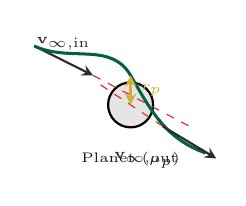
\begin{tikzpicture}[scale=0.68]
                    \draw[thick, fill=gray!20] (0,0) circle (0.42cm);
                    \node[below=0.48cm, font=\tiny, color=DarkSlate] at (0,0) {Planet ($\mu_p$)};
                    
                    \draw[thick, ->, >=stealth, color=Charcoal, line width=0.8pt] (-1.8, 1.1) -- (-0.7, 0.55) node[midway, above, font=\tiny]{$\mathbf{v}_{\infty,\text{in}}$};
                    \draw[thick, color=UdeAGreen, line width=1.1pt] (-1.8, 1.1) to[out=-25, in=120] (0, 0.55) to[out=-60, in=160] (1.4, -0.9);
                    \draw[thick, ->, >=stealth, color=Charcoal, line width=0.8pt] (0.6, -0.4) -- (1.6, -1.0) node[midway, below left, font=\tiny]{$\mathbf{v}_{\infty,\text{out}}$};
                    \draw[dashed, color=AlertRed] (-0.7, 0.55) -- (1.1, -0.4);
                    \draw[dashed, color=AlertRed] (0.6, -0.4) -- (-0.6, 0.4);
                    \draw[<->, >=stealth, color=UdeAGold, line width=0.8pt] (0,0) -- (0,0.55) node[midway, right, font=\tiny]{$r_p$};
                \end{tikzpicture}
            \end{block}
            \vspace{-0.1cm}
            \begin{alertblock}{Feasibility Bound}
                \scriptsize $r_p \ge R_{\text{planet}} + h_{\text{atm,safe}}$ limits max turn $\delta_{\text{turn,max}}$.
            \end{alertblock}
        \end{column}
    \end{columns}
\end{frame}

% ==============================================================================
% SLIDE 28: HELIOCENTRIC MOMENTUM & OBERTH
% ==============================================================================
\begin{frame}{Heliocentric Momentum Transfer and Powered Flybys}
    \begin{columns}[t]
        \begin{column}{0.48\textwidth}
            \begin{block}{Heliocentric Energy Exchange}
                \scriptsize
                \begin{equation*}
                    \mathbf{v}_{\odot,\text{out}} = \mathbf{v}_{\text{planet}} + \mathbf{v}_{\infty,\text{out}}
                \end{equation*}
                \vspace{-0.15cm}
                Net heliocentric velocity change:
                \begin{equation*}
                    \|\Delta \mathbf{V}_{\odot}\| = 2 v_\infty \sin\left(\frac{\delta_{\text{turn}}}{2}\right)
                \end{equation*}
                \vspace{-0.15cm}
                \begin{itemize}\setlength{\itemsep}{1pt}
                    \item \textbf{Trailing-Side:} Crosses behind planet $\implies \Delta E_\odot > 0$ (Speed Boost).
                    \item \textbf{Leading-Side:} Crosses in front of planet $\implies \Delta E_\odot < 0$ (Gravity Brake).
                \end{itemize}
            \end{block}
        \end{column}

        \begin{column}{0.48\textwidth}
            \begin{alertblock}{The Deep-Space Oberth Effect}
                \scriptsize
                Executing burn $\Delta v_p$ at periapsis $r_p$:
                \begin{align*}
                    v_{p,-} &= \sqrt{v_\infty^2 + \frac{2\mu_p}{r_p}} \\
                    v_{\infty,\text{out}} &= \sqrt{(v_{p,-} + \Delta v_p)^2 - \frac{2\mu_p}{r_p}}
                \end{align*}
                \vspace{-0.15cm}
                \textbf{Kinetic Energy Lever Arm:}
                \begin{equation*}
                    \Delta E_k \approx v_{p,-}\Delta v_p \gg v_\infty \Delta v_p
                \end{equation*}
                \vspace{-0.05cm}
                Periapsis burns maximize excess velocity gains!
            \end{alertblock}
        \end{column}
    \end{columns}
\end{frame}

% ==============================================================================
% SLIDE 29: WORKED EXAMPLE 2 (VOYAGER 2)
% ==============================================================================
\begin{frame}{Worked Example 2: Voyager 2 Jupiter Gravity Assist}
    \begin{exampleblock}{Jupiter Encounter Benchmark}
        \scriptsize
        Voyager 2 approaches Jupiter ($\mu_J = 1.26686 \times 10^8\text{ km}^3/\text{s}^2$, $R_J = 71492\text{ km}$) with $v_\infty = 10.60\text{ km/s}$ at $r_p = 5.0\,R_J = 357460\text{ km}$.
    \end{exampleblock}

    \vspace{-0.15cm}

    \begin{columns}[t]
        \begin{column}{0.48\textwidth}
            \scriptsize
            \textbf{Step 1: Eccentricity and Turning Angle}
            \begin{align*}
                e &= 1 + \frac{r_p v_\infty^2}{\mu_J} = 1 + \frac{(357460)(10.60)^2}{1.26686 \times 10^8} = 1.317 \\
                \sin\left(\frac{\delta}{2}\right) &= \frac{1}{1.317} = 0.7593 \implies \delta_{\text{turn}} = \mathbf{98.81}^\circ
            \end{align*}
            \vspace{-0.15cm}
            \textbf{Step 2: Periapsis Velocity}
            \begin{equation*}
                v_p = \sqrt{10.60^2 + \frac{2(1.26686 \times 10^8)}{357460}} = \mathbf{28.65}\text{ km/s}
            \end{equation*}
        \end{column}

        \begin{column}{0.48\textwidth}
            \scriptsize
            \textbf{Step 3: Heliocentric Flyby $\Delta \mathbf{V}_\odot$}
            \begin{equation*}
                \|\Delta \mathbf{V}_{\odot}\| = 2(10.60)\sin(49.40^\circ) = \mathbf{16.10}\text{ km/s}
            \end{equation*}
            \textbf{Step 4: Energy Audit}
            \begin{itemize}\setlength{\itemsep}{1pt}
                \item Delivering $16.10\text{ km/s}$ chemically requires propellant mass fraction $>99.5\%$.
                \item Gravity assist delivers this velocity gain \textbf{propellant-free}.
            \end{itemize}
        \end{column}
    \end{columns}
\end{frame}

% ==============================================================================
% SLIDE 30: PYTHON CODE: GRAVITY ASSIST & OBERTH KINEMATICS
% ==============================================================================
\begin{frame}[fragile]{Python Implementation: Gravity Assist and Oberth Kinematics}
    \begin{columns}[t]
        \begin{column}{0.48\textwidth}
            \begin{block}{Flyby Vector Kinematics}
                \scriptsize
                The Python function solves:
                \begin{itemize}\setlength{\itemsep}{1.5pt}
                    \item Turning angle $\delta_{\text{turn}} = 2 \arcsin(1 / (1 + r_p v_\infty^2 / \mu_p))$.
                    \item Net heliocentric impulse $\|\Delta \mathbf{V}_\odot\| = 2 v_\infty \sin(\delta_{\text{turn}}/2)$.
                    \item Periapsis burn Oberth amplification:
                    \begin{equation*}
                        v_{\infty,\text{out}} = \sqrt{(v_p + \Delta v_p)^2 - 2\mu_p / r_p}
                    \end{equation*}
                    \item Quantifies equivalent chemical propellant mass saved via Tsiolkovsky equation.
                \end{itemize}
            \end{block}
        \end{column}

        \begin{column}{0.50\textwidth}
\begin{lstlisting}[style=pythoncode]
import numpy as np

def compute_gravity_assist(mu_planet, R_planet, rp_km, v_inf_in, dv_p=0.0):
    # Hyperbolic parameters
    e = 1.0 + (rp_km * v_inf_in**2) / mu_planet
    turn_angle_rad = 2.0 * np.arcsin(1.0 / e)
    
    # Heliocentric impulse (ballistic flyby)
    dV_helio = 2.0 * v_inf_in * np.sin(turn_angle_rad / 2.0)
    
    # Periapsis velocity before burn
    vp_in = np.sqrt(v_inf_in**2 + (2.0 * mu_planet) / rp_km)
    
    # Powered Oberth flyby
    vp_out = vp_in + dv_p
    v_inf_out = np.sqrt(vp_out**2 - (2.0 * mu_planet) / rp_km)
    
    return {
        "eccentricity": e,
        "delta_turn_deg": np.degrees(turn_angle_rad),
        "dV_helio_boost": dV_helio,
        "vp_km_s": vp_in,
        "v_inf_out": v_inf_out
    }
\end{lstlisting}
        \end{column}
    \end{columns}
\end{frame}

% ==============================================================================
% SLIDE 31: HISTORICAL MULTI-FLYBY MISSIONS
% ==============================================================================
\begin{frame}{Historical Gravity Assists: Expanding Solar System Reach}
    \begin{columns}[t]
        \begin{column}{0.48\textwidth}
            \begin{block}{Why Multi-Flyby Trajectories?}
                \scriptsize
                Gravity assists add momentum to a spacecraft far beyond chemical propulsion limits:
                \begin{itemize}\setlength{\itemsep}{1.5pt}
                    \item \textbf{Voyager 1 and 2 (1977):} Leveraged a rare alignment of Jupiter and Saturn to achieve solar system escape velocity.
                    \item \textbf{Galileo (1989):} Used a \textbf{VEEGA} (Venus-Earth-Earth Gravity Assist) trajectory after Shuttle payload limits were revised.
                \end{itemize}
            \end{block}
        \end{column}

        \begin{column}{0.48\textwidth}
            \begin{exampleblock}{Cassini-Huygens (1997)}
                \scriptsize
                Reached Saturn in 2004 via a 4-flyby \textbf{VVEJGA} architecture (Venus-Venus-Earth-Jupiter):
                \begin{itemize}\setlength{\itemsep}{1.5pt}
                    \item Venus Flyby 1 (1998): $+7.0\text{ km/s}$
                    \item Venus Flyby 2 (1999): $+5.5\text{ km/s}$
                    \item Earth Flyby (1999): $+5.5\text{ km/s}$
                    \item Jupiter Flyby (2000): $+2.2\text{ km/s}$
                \end{itemize}
                Delivered $\sim 20\text{ km/s}$ of free $\Delta V$, impossible with any single launch vehicle!
            \end{exampleblock}
        \end{column}
    \end{columns}
\end{frame}

% ==============================================================================
% SLIDE 32: B-PLANE FOUNDATIONS
% ==============================================================================
\begin{frame}{Week 7: The B-Plane Targeting Framework --- Foundations}
    \begin{columns}[t]
        \begin{column}{0.54\textwidth}
            \begin{block}{Why Direct Targeting Fails in Deep Space}
                \scriptsize
                \begin{itemize}\setlength{\itemsep}{1pt}
                    \item Propagating to fixed $t_f$ is ill-conditioned: a 1-second timing error causes $>30\text{ km}$ miss distance.
                    \item \textbf{Solution:} B-Plane target disk passes through body center, perpendicular to incoming asymptote $\mathbf{v}_\infty$.
                \end{itemize}
            \end{block}
            \begin{block}{Orthonormal Basis $(\hat{\mathbf{S}}, \hat{\mathbf{T}}, \hat{\mathbf{R}})$}
                \scriptsize
                \begin{equation*}
                    \hat{\mathbf{S}} = \frac{\mathbf{v}_\infty}{\|\mathbf{v}_\infty\|}, \quad
                    \hat{\mathbf{T}} = \frac{\hat{\mathbf{S}} \times \hat{\mathbf{k}}}{\|\hat{\mathbf{S}} \times \hat{\mathbf{k}}\|}, \quad
                    \hat{\mathbf{R}} = \hat{\mathbf{S}} \times \hat{\mathbf{T}}
                \end{equation*}
                where $\hat{\mathbf{k}}$ is reference normal (e.g., Ecliptic North).
            \end{block}
        \end{column}

        \begin{column}{0.43\textwidth}
            \begin{block}{B-Plane Geometry}
                \centering
                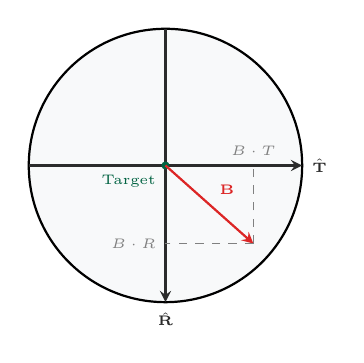
\begin{tikzpicture}[scale=0.62]
                    \draw[thick, fill=LightBg] (0,0) circle (2.8cm);
                    \draw[thick, ->, >=stealth, color=Charcoal] (-2.8,0) -- (2.8,0) node[right, font=\tiny]{$\hat{\mathbf{T}}$};
                    \draw[thick, ->, >=stealth, color=Charcoal] (0,2.8) -- (0,-2.8) node[below, font=\tiny]{$\hat{\mathbf{R}}$};
                    \filldraw[color=UdeAGreen] (0,0) circle (2pt) node[below left, font=\tiny]{Target};
                    \draw[thick, ->, >=stealth, color=AlertRed, line width=0.8pt] (0,0) -- (1.8,-1.6) node[midway, above right, font=\tiny]{$\mathbf{B}$};
                    \draw[dashed, color=gray] (1.8,-1.6) -- (1.8,0) node[above, font=\tiny]{$B\cdot T$};
                    \draw[dashed, color=gray] (1.8,-1.6) -- (0,-1.6) node[left, font=\tiny]{$B\cdot R$};
                \end{tikzpicture}
            \end{block}
        \end{column}
    \end{columns}
\end{frame}

% ==============================================================================
% SLIDE 33: B-PLANE PARAMETERS (REVISED FOR ZERO OVERFLOW)
% ==============================================================================
\begin{frame}{B-Plane Target Quantities and Impact Parameter Derivations}
    \begin{columns}[t]
        \begin{column}{0.48\textwidth}
            \begin{block}{Impact Parameter Vector $\mathbf{B}$}
                \scriptsize
                Miss vector on the B-plane:
                \par\vspace{1pt}
                {\centering $\mathbf{B} = (B \cdot T)\hat{\mathbf{T}} + (B \cdot R)\hat{\mathbf{R}}$\par}
                \vspace{1pt}
                where $B \cdot T = B \cos \theta_B$ and $B \cdot R = B \sin \theta_B$.
                \par\vspace{3pt}
                \textbf{Impact Parameter Magnitude ($B = \Vert{}\mathbf{B}\Vert{}$):}
                \par\vspace{1pt}
                {\centering $\displaystyle B = r_p \sqrt{1 + \frac{2\mu_p}{r_p v_\infty^2}} = \frac{\mu_p}{v_\infty^2}\sqrt{e^2 - 1}$\par}
            \end{block}
        \end{column}

        \begin{column}{0.48\textwidth}
            \begin{alertblock}{Linearized State Transition Mapping}
                \scriptsize
                For mid-course TCM burn $\Delta \mathbf{v}_{\text{TCM}}$ at epoch $t_{\text{TCM}}$:
                \par\vspace{1pt}
                {\centering $\displaystyle \begin{bmatrix} \Delta(B \cdot T) \\ \Delta(B \cdot R) \\ \Delta \text{TIF} \end{bmatrix} = \left[ \frac{\partial \mathbf{B}}{\partial \mathbf{r}(t_f)} \boldsymbol{\Phi}_{r v}(t_f, t_{\text{TCM}}) \right] \Delta \mathbf{v}_{\text{TCM}}$\par}
                \vspace{1pt}
                where $\text{TIF}$ is Time to Intercept and $\boldsymbol{\Phi}_{rv}$ is the STM partition.
                \begin{itemize}\setlength{\itemsep}{1pt}\setlength{\topsep}{1pt}
                    \item Inverting the sensitivity matrix yields exact 3-axis TCM commands.
                \end{itemize}
            \end{alertblock}
        \end{column}
    \end{columns}
\end{frame}

% ==============================================================================
% SLIDE 34: WORKED EXAMPLE: B-PLANE TARGET SIZING
% ==============================================================================
\begin{frame}{Worked Example: B-Plane Target Vector Sizing at Mars}
    \begin{exampleblock}{Mission Specification}
        \scriptsize
        A science probe approaches Mars ($\mu_M = 42828.37\text{ km}^3/\text{s}^2$, $R_M = 3396.2\text{ km}$) with $v_\infty = 3.50\text{ km/s}$[cite: 1, 15]. \\
        Design a polar capture flyby with periapsis altitude $h_p = 300\text{ km}$ ($r_p = 3696.2\text{ km}$) and zero out-of-plane azimuth ($\theta_B = 270^\circ$).
    \end{exampleblock}

    \vspace{-0.15cm}

    \begin{columns}[t]
        \begin{column}{0.48\textwidth}
            \scriptsize
            \textbf{Step 1: Hyperbolic Eccentricity ($e$)}
            \begin{align*}
                e &= 1 + \frac{r_p v_\infty^2}{\mu_M} = 1 + \frac{(3696.2)(3.50)^2}{42828.37} = \mathbf{2.057}
            \end{align*}
            \textbf{Step 2: Impact Parameter Magnitude ($B$)}
            \begin{align*}
                B &= r_p \sqrt{1 + \frac{2\mu_M}{r_p v_\infty^2}} = 3696.2 \sqrt{1 + \frac{2(42828.37)}{(3696.2)(12.25)}} \\
                &= 3696.2 \sqrt{1 + 1.891} = 3696.2(1.700) = \mathbf{6284.8\text{ km}}
            \end{align*}
        \end{column}

        \begin{column}{0.48\textwidth}
            \scriptsize
            \textbf{Step 3: Target Coordinates on the B-Plane}
            \begin{align*}
                B\cdot T &= B \cos(270^\circ) = \mathbf{0.0\text{ km}} \\
                B\cdot R &= B \sin(270^\circ) = \mathbf{-6284.8\text{ km}}
            \end{align*}
            \textbf{Step 4: Forensic Insight for GMAT Targeter}
            \begin{itemize}\setlength{\itemsep}{1pt}
                \item Pure polar arrival: All miss vector projected along the $-\hat{\mathbf{R}}$ axis.
                \item Direct inputs for GMAT:
                \begin{itemize}
                    \item \texttt{MarsInertial.BdotT = 0.0}
                    \item \texttt{MarsInertial.BdotR = -6284.8}
                \end{itemize}
            \end{itemize}
        \end{column}
    \end{columns}
\end{frame}

% ==============================================================================
% SLIDE: IVP VS. BVP IN ASTRODYNAMICS (CORRECTED FIT)
% ==============================================================================
\begin{frame}{The Astrodynamic Duality: Initial Value vs. Boundary Value Problems}
    \begin{columns}[t]
        \begin{column}{0.54\textwidth}
            \begin{block}{Initial Value Problem (IVP: Forward Simulation)}
                \scriptsize
                Given the full state at epoch $t_0$, determine downstream motion:
                \par\vspace{1pt}
                {\centering $\mathbf{x}(t_0) = [\mathbf{r}_0^T, \mathbf{v}_0^T]^T \xrightarrow{\text{Integrate}} \dot{\mathbf{x}} = \mathbf{f}(\mathbf{x}, t) \to \mathbf{x}(t)$\par}
                \vspace{2pt}
                \begin{itemize}\setlength{\itemsep}{1pt}\setlength{\topsep}{0pt}\setlength{\parsep}{0pt}
                    \item Deterministic, fast, and stable (standard RK4/78 solvers).
                    \item \textbf{Operational flaw:} Required initial velocity $\mathbf{v}_0$ is unknown a priori.
                \end{itemize}
            \end{block}

            \vspace{-0.08cm}

            \begin{block}{Boundary Value Problem (BVP: The Targeter)}
                \scriptsize
                Constraints are partitioned across distinct temporal endpoints:
                \par\vspace{1pt}
                {\centering $\mathbf{r}(t_0) = \mathbf{r}_{\text{launch}} \quad \text{and} \quad \mathbf{r}(t_f) = \mathbf{r}_{\text{target}} \quad (\text{or } \mathbf{B}^*)$\par}
                \vspace{2pt}
                \begin{itemize}\setlength{\itemsep}{1pt}\setlength{\topsep}{0pt}\setlength{\parsep}{0pt}
                    \item \textbf{Core Question:} \textit{What initial $\mathbf{v}_0$ (or $\Delta \mathbf{V}$) connects both endpoints?}
                    \item Non-linear: cannot be integrated in a single forward pass.
                \end{itemize}
            \end{block}
        \end{column}

        \begin{column}{0.43\textwidth}
            \begin{block}{Endpoint Constraint Geometry}
                \centering
                \vspace{0.05cm}
                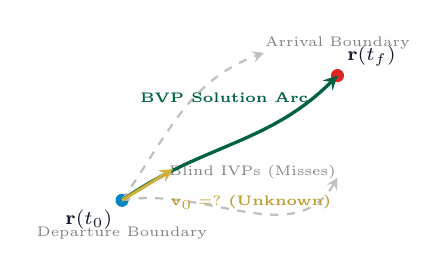
\begin{tikzpicture}[scale=0.72, >=stealth]
                    % Origin / Earth
                    \filldraw[color=SpiceBlue] (-2.0, -1.0) circle (3pt);
                    \node[below left, font=\scriptsize\bfseries, color=DarkSlate] at (-2.0, -1.0) {$\mathbf{r}(t_0)$};
                    \node[below=6pt, font=\tiny, color=gray] at (-2.0, -1.0) {Departure Boundary};

                    % Target / Destination
                    \filldraw[color=AlertRed] (1.8, 1.2) circle (3pt);
                    \node[above right, font=\scriptsize\bfseries, color=DarkSlate] at (1.8, 1.2) {$\mathbf{r}(t_f)$};
                    \node[above=6pt, font=\tiny, color=gray] at (1.8, 1.2) {Arrival Boundary};

                    % Forward IVP guesses (Misses)
                    \draw[thick, color=gray!50, dashed, ->] (-2.0, -1.0) to[out=55, in=-160] (0.5, 1.6);
                    \draw[thick, color=gray!50, dashed, ->] (-2.0, -1.0) to[out=10, in=-120] (1.8, -0.6);
                    \node[font=\tiny, color=gray] at (0.3, -0.5) {Blind IVPs (Misses)};

                    % The Connecting BVP Arc
                    \draw[very thick, color=UdeAGreen, ->] (-2.0, -1.0) to[out=35, in=-135] (1.8, 1.2);
                    \node[above=2pt, sloped, font=\tiny\bfseries, color=UdeAGreen] at (-0.2, 0.45) {BVP Solution Arc};

                    % Unknown Velocity Vector
                    \draw[thick, color=UdeAGold, ->, line width=1.1pt] (-2.0, -1.0) -- (-1.1, -0.45);
                    \node[below right=1pt, font=\tiny\bfseries, color=UdeAGold!90!black] at (-1.35, -0.7) {$\mathbf{v}_0 = ?$ (Unknown)};
                \end{tikzpicture}
            \end{block}

            \vspace{-0.1cm}

            \begin{alertblock}{The Astrodynamic Dilemma}
                \scriptsize
                Missions are dictated by \textbf{where we must arrive}, not by where an arbitrary velocity vector happens to drop us.
            \end{alertblock}
        \end{column}
    \end{columns}
\end{frame}

% ==============================================================================
% SLIDE: WHY BVPS ARE INESCAPABLE IN REAL TRAJECTORIES
% ==============================================================================
\begin{frame}{Why Boundary Value Problems are Inescapable in Deep-Space Flight}
    \begin{columns}[t]
        \begin{column}{0.50\textwidth}
            \begin{block}{1. Astronomical Independence of Planetary Motion}
                \scriptsize
                \begin{itemize}\setlength{\itemsep}{1.5pt}
                    \item Earth and target bodies travel on independent, eccentric, inclined heliocentric orbits.
                    \item Launch calendar and arrival science windows fix the \textbf{position endpoints} $(\mathbf{r}_1, \mathbf{r}_2)$ and flight duration $\Delta t$.
                    \item The velocity vector $\mathbf{v}_1$ is a free dependent variable that must be calculated to satisfy Kepler's boundary equation.
                \end{itemize}
            \end{block}

            \vspace{-0.08cm}

            \begin{block}{2. The Non-Integrability Barrier ($N$-Body Universe)}
                \scriptsize
                \begin{itemize}\setlength{\itemsep}{1.5pt}
                    \item Classical Lambert algorithms solve the idealized 2-body BVP.
                    \item Real flight entails third-body gravity (Sun, Jupiter, Moon), non-spherical geopotentials ($J_2, C_{nm}$), and solar radiation pressure.
                    \item The operational equations of motion have \textbf{no closed-form analytical solution}; endpoint matching requires numerical BVPs.
                \end{itemize}
            \end{block}
        \end{column}

        \begin{column}{0.48\textwidth}
            \begin{block}{3. Critical Terminal Entry Corridors}
                \scriptsize
                Targeting margins at interplanetary arrival are zero:
                \begin{itemize}\setlength{\itemsep}{1.5pt}
                    \item \textbf{Atmospheric Entry (e.g., Mars 2020):} Flight path angle corridor is narrow ($\gamma \pm 0.10^\circ$) to avoid burnup or skip-out.
                    \item \textbf{Planetary Capture:} Retrograde $\Delta v_{\text{cap}}$ requires periapsis precision within tens of kilometers.
                    \item \textbf{Gravity Assists:} Turning angle $\delta_{\text{turn}}$ depends non-linearly on hyperbola flyby altitude $r_p$.
                \end{itemize}
            \end{block}

            \vspace{-0.08cm}

            \begin{alertblock}{The Mathematical Mandate}
                \scriptsize
                Because forward intuition cannot invert non-linear gravitational dynamics, navigators must formulate:
                \vspace{-0.05cm}
                \begin{equation*}
                    \mathbf{F}(\mathbf{v}_0) = \mathbf{r}(t_f; \mathbf{v}_0) - \mathbf{r}_{\text{target}}(t_f) = \mathbf{0}
                \end{equation*}
                \vspace{-0.01cm}
                This root-finding condition necessitates \textbf{shooting solvers and differential correctors}.
            \end{alertblock}
        \end{column}
    \end{columns}
\end{frame}

% ==============================================================================
% SLIDE 35: NUMERICAL BOUNDARY SOLVERS (ENLARGED FORWARD SHOOTING DIAGRAM)
% ==============================================================================
\begin{frame}{Numerical Boundary Solvers: The Shooting Method Architecture}
    \begin{columns}[t]
        \begin{column}{0.48\textwidth}
            \begin{block}{Two-Point Boundary Value Problem (TPBVP)}
                \scriptsize
                Interplanetary trajectory design is formulated as a boundary value problem:
                \begin{itemize}\setlength{\itemsep}{2pt}\setlength{\topsep}{1pt}
                    \item \textbf{Control Vector ($\mathbf{X} \in \mathbb{R}^n$):} Unknown initial/maneuver parameters (e.g., burn components $\Delta V_x, \Delta V_y, \Delta V_z$).
                    \item \textbf{Goal Vector ($\mathbf{Y} \in \mathbb{R}^m$):} Constrained terminal conditions (e.g., $B\cdot T, B\cdot R$, arrival epoch $t_f$).
                \end{itemize}
            \end{block}

            \vspace{-0.1cm}

            \begin{alertblock}{Iterative Convergence Criterion}
                \scriptsize
                Trajectories shoot forward in time until miss distance converges:
                \par\vspace{2pt}
                {\centering $\|\mathbf{Y}(\mathbf{X}_k) - \mathbf{Y}^*\| \le \boldsymbol{\epsilon}_{\text{tol}}$\par}
            \end{alertblock}
        \end{column}

        \begin{column}{0.50\textwidth}
            \begin{block}{The Forward Shooting Mechanism}
                \centering
                \vspace{0.15cm}
                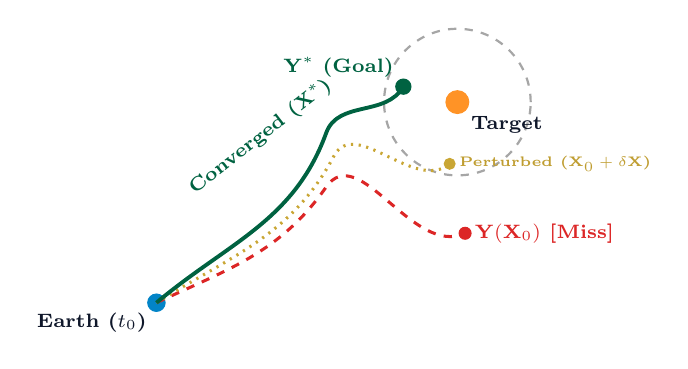
\begin{tikzpicture}[scale=0.98, >=stealth]
                    % Departure Node (Earth)
                    \filldraw[color=SpiceBlue] (-2.2, -1.2) circle (3.2pt);
                    \node[below left, font=\scriptsize\bfseries, color=DarkSlate] at (-2.2, -1.2) {Earth ($t_0$)};
                    
                    % Target Body & Capture Region
                    \draw[dashed, color=gray!70, line width=0.8pt] (1.7, 1.4) circle (0.95cm);
                    \filldraw[color=orange!85] (1.7, 1.4) circle (4.2pt) node[below right=2pt, font=\scriptsize\bfseries, color=DarkSlate]{Target};
                    
                    % Goal Point Y*
                    \filldraw[color=UdeAGreen] (1.0, 1.6) circle (2.8pt);
                    \node[above left, font=\scriptsize\bfseries, color=UdeAGreen] at (1.0, 1.6) {$\mathbf{Y}^*$ (Goal)};
                    
                    % Trajectory 0: Initial Nominal Miss
                    \draw[thick, color=AlertRed, dashed, line width=1.1pt] (-2.2, -1.2) to[out=25, in=-125] (0.0, 0.3) to[out=55, in=-155] (1.8, -0.3);
                    \filldraw[color=AlertRed] (1.8, -0.3) circle (2.2pt);
                    \node[right, font=\scriptsize\bfseries, color=AlertRed] at (1.8, -0.3) {$\mathbf{Y}(\mathbf{X}_0)$ [Miss]};
                    
                    % Trajectory 1: Perturbed Gradient Step
                    \draw[thick, color=UdeAGold!95!black, dotted, line width=1.1pt] (-2.2, -1.2) to[out=32, in=-118] (0.1, 0.7) to[out=62, in=-140] (1.6, 0.6);
                    \filldraw[color=UdeAGold!95!black] (1.6, 0.6) circle (2.0pt);
                    \node[right, font=\tiny\bfseries, color=UdeAGold!90!black] at (1.6, 0.6) {Perturbed ($\mathbf{X}_0 + \delta \mathbf{X}$)};
                    
                    % Trajectory 2: Converged Solution
                    \draw[very thick, color=UdeAGreen, line width=1.4pt] (-2.2, -1.2) to[out=40, in=-110] (0.0, 1.0) to[out=70, in=-120] (1.0, 1.6);
                    \node[color=UdeAGreen, font=\scriptsize\bfseries, rotate=38] at (-0.85, 0.95) {Converged ($\mathbf{X}^*$)};
                \end{tikzpicture}
                \vspace{0.15cm}
            \end{block}
        \end{column}
    \end{columns}
\end{frame}

% ==============================================================================
% SLIDE 36: DIFFERENTIAL CORRECTOR (SPLIT PART 2: JACOBIAN & UPDATE)
% ==============================================================================
\begin{frame}{The Differential Corrector: Newton-Raphson Jacobian Formulation}
    \begin{columns}[t]
        \begin{column}{0.50\textwidth}
            \begin{block}{Linearizing State Transitions: The Jacobian ($\mathbf{J}$)}
                \scriptsize
                The Differential Corrector builds the sensitivity matrix $\mathbf{J}$ via finite difference perturbations:
                \vspace{-0.05cm}
                \begin{equation*}
                    \mathbf{J} = \begin{bmatrix}
                        \frac{\partial Y_1}{\partial X_1} & \cdots & \frac{\partial Y_1}{\partial X_n} \\
                        \vdots & \ddots & \vdots \\
                        \frac{\partial Y_m}{\partial X_1} & \cdots & \frac{\partial Y_m}{\partial X_n}
                    \end{bmatrix}, \quad 
                    J_{ij} \approx \frac{Y_i(\mathbf{X} + \delta X_j \hat{\mathbf{e}}_j) - Y_i(\mathbf{X})}{\delta X_j}
                \end{equation*}
                \vspace{-0.15cm}
                \begin{itemize}\setlength{\itemsep}{1pt}
                    \item Each Jacobian evaluation requires $n+1$ forward trajectory numerical integrations.
                \end{itemize}
            \end{block}
        \end{column}

        \begin{column}{0.47\textwidth}
            \begin{block}{Newton-Raphson Parameter Step}
                \scriptsize
                For square problems ($m = n$), the parameter update vector is:
                \par\vspace{1pt}
                {\centering $\mathbf{X}_{k+1} = \mathbf{X}_k - \mathbf{J}^{-1} \left(\mathbf{Y}(\mathbf{X}_k) - \mathbf{Y}^*\right)$\par}
                \vspace{2pt}
                For over-determined problems ($n > m$), GMAT employs pseudo-inverse minimum-norm updates:
                \par\vspace{1pt}
                {\centering $\Delta \mathbf{X} = -\mathbf{J}^T (\mathbf{J} \mathbf{J}^T)^{-1} \left(\mathbf{Y} - \mathbf{Y}^*\right)$\par}
            \end{block}

            \vspace{-0.1cm}

            \begin{alertblock}{Condition Number Check}
                \scriptsize If $\det(\mathbf{J}) \approx 0$, the targeter is singular. Control inputs must have non-zero gradient projections onto goals.
            \end{alertblock}
        \end{column}
    \end{columns}
\end{frame}

% ==============================================================================
% SLIDE A: NEWTON-RAPHSON IN GMAT DIFFERENTIAL CORRECTOR
% ==============================================================================
\begin{frame}{GMAT Differential Corrector: Full Newton-Raphson Algorithm}
    \begin{columns}[t]
        \begin{column}{0.52\textwidth}
            \begin{block}{Exact Gradient Re-evaluation Principle}
                \scriptsize
                The standard \texttt{NewtonRaphson} algorithm reconstructs the full sensitivity Jacobian $\mathbf{J}_k \in \mathbb{R}^{m \times n}$ at \textbf{every iteration} $k$ via finite differences[cite: 9]:
                \par\vspace{2pt}
                {\centering $\displaystyle J_{ij} \approx \frac{Y_i(\mathbf{X}_k + \delta X_j \hat{\mathbf{e}}_j) - Y_i(\mathbf{X}_k)}{\delta X_j}$\par}
                \vspace{2pt}
                \begin{itemize}\setlength{\itemsep}{1.2pt}\setlength{\topsep}{0pt}
                    \item Parameter update step:
                    \par\vspace{1pt}
                    {\centering $\displaystyle \Delta \mathbf{X}_k = -\mathbf{J}_k^{-1} \left(\mathbf{Y}(\mathbf{X}_k) - \mathbf{Y}^*\right)$\par}
                    \item Guarantees local \textbf{quadratic convergence} ($\|\mathbf{e}_{k+1}\| \propto \|\mathbf{e}_k\|^2$) near the root.
                    \item Reaches convergence in the fewest number of solver iterations (typically 2--4 iterations).
                \end{itemize}
            \end{block}

            \vspace{-0.08cm}

            \begin{alertblock}{The Computational Bottleneck}
                \scriptsize
                For $n$ control variables, assembling $\mathbf{J}_k$ demands:
                \par\vspace{1pt}
                {\centering $\text{Propagations per iteration} = n + 1$\par}
                In high-fidelity interplanetary flight (numerical $N$-body, SRP, $J_2$), re-propagating $n+1$ trajectories every step dominates CPU runtime.
            \end{alertblock}
        \end{column}

        \begin{column}{0.45\textwidth}
            \begin{block}{Newton-Raphson Iteration Cost}
                \centering
                \vspace{0.1cm}
                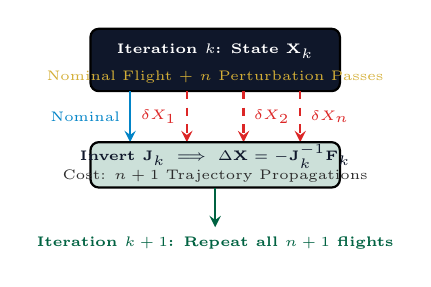
\begin{tikzpicture}[scale=0.72, >=stealth]
                    % Step k box
                    \draw[thick, fill=DarkSlate, rounded corners=3pt] (-2.2, 1.8) rectangle (2.2, 0.7);
                    \node[color=white, font=\tiny\bfseries] at (0, 1.4) {Iteration $k$: State $\mathbf{X}_k$};
                    \node[color=UdeAGold, font=\fontsize{5pt}{6pt}\selectfont] at (0, 0.95) {Nominal Flight + $n$ Perturbation Passes};

                    % Arrows representing n+1 flights
                    \draw[thick, color=SpiceBlue, ->] (-1.5, 0.7) -- (-1.5, -0.2) node[midway, left, font=\fontsize{4.5pt}{5pt}\selectfont]{Nominal};
                    \draw[thick, color=AlertRed, dashed, ->] (-0.5, 0.7) -- (-0.5, -0.2) node[midway, left, font=\fontsize{4.5pt}{5pt}\selectfont]{$\delta X_1$};
                    \draw[thick, color=AlertRed, dashed, ->] (0.5, 0.7) -- (0.5, -0.2) node[midway, right, font=\fontsize{4.5pt}{5pt}\selectfont]{$\delta X_2$};
                    \draw[thick, color=AlertRed, dashed, ->] (1.5, 0.7) -- (1.5, -0.2) node[midway, right, font=\fontsize{4.5pt}{5pt}\selectfont]{$\delta X_n$};

                    % Inversion block
                    \draw[thick, fill=UdeAGreen!20, rounded corners=3pt] (-2.2, -0.2) rectangle (2.2, -1.0);
                    \node[color=DarkSlate, font=\tiny\bfseries] at (0, -0.45) {Invert $\mathbf{J}_k \implies \Delta \mathbf{X} = -\mathbf{J}_k^{-1} \mathbf{F}_k$};
                    \node[color=Charcoal, font=\fontsize{5pt}{6pt}\selectfont] at (0, -0.8) {Cost: $n+1$ Trajectory Propagations};

                    % Next step arrow
                    \draw[thick, color=UdeAGreen, ->] (0, -1.0) -- (0, -1.7);
                    \node[below, font=\tiny\bfseries, color=UdeAGreen] at (0, -1.7) {Iteration $k+1$: Repeat all $n+1$ flights};
                \end{tikzpicture}
            \end{block}

            \vspace{-0.1cm}

            \begin{exampleblock}{Recommended Use in GMAT}
                \scriptsize
                Best for simple transfers ($n \le 3$), highly non-linear orbital regimes, or when initial guesses are poor[cite: 3].
            \end{exampleblock}
        \end{column}
    \end{columns}
\end{frame}

% ==============================================================================
% SLIDE B: BROYDEN'S QUASI-NEWTON METHOD IN GMAT
% ==============================================================================
\begin{frame}{GMAT Differential Corrector: Broyden's Quasi-Newton Method}
    \begin{columns}[t]
        \begin{column}{0.53\textwidth}
            \begin{block}{Rank-1 Secant Matrix Update Principle}
                \scriptsize
                The \texttt{Broyden} algorithm replaces expensive derivative flights with a multi-dimensional secant approximation[cite: 9]:
                \begin{itemize}\setlength{\itemsep}{1.2pt}\setlength{\topsep}{0pt}
                    \item \textbf{Iteration $k = 0$:} Computes initial $\mathbf{B}_0 \approx \mathbf{J}_0$ using finite-difference perturbation passes ($n+1$ propagations).
                    \item \textbf{Iterations $k \ge 1$:} Uses trajectory telemetry from the previous step to update $\mathbf{B}_k$ with \textbf{zero perturbation flights}:
                    \par\vspace{1pt}
                    {\centering $\displaystyle \mathbf{B}_{k+1} = \mathbf{B}_k + \frac{\left(\Delta \mathbf{F}_k - \mathbf{B}_k \Delta \mathbf{X}_k\right) \Delta \mathbf{X}_k^T}{\Delta \mathbf{X}_k^T \Delta \mathbf{X}_k}$\par}
                    where $\Delta \mathbf{X}_k = \mathbf{X}_{k+1} - \mathbf{X}_k$ and $\Delta \mathbf{F}_k = \mathbf{F}_{k+1} - \mathbf{F}_k$.
                \end{itemize}
            \end{block}

            \vspace{-0.08cm}

            \begin{exampleblock}{The Numerical Payoff: 1 Propagation per Step}
                \scriptsize
                After iteration 0, \textbf{each iteration requires only 1 forward trajectory integration}!
                \begin{itemize}\setlength{\itemsep}{0.8pt}
                    \item Achieves \textbf{superlinear convergence} rate.
                    \item May require 1--2 more iterations than Newton-Raphson, but cuts total trajectory propagations by up to $60\%$.
                \end{itemize}
            \end{exampleblock}
        \end{column}

        \begin{column}{0.44\textwidth}
            \begin{block}{Broyden Secant Efficiency}
                \centering
                \vspace{0.1cm}
                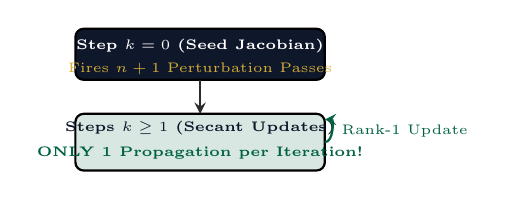
\begin{tikzpicture}[scale=0.72, >=stealth]
                    % Step 0
                    \draw[thick, fill=DarkSlate, rounded corners=3pt] (-2.2, 1.8) rectangle (2.2, 0.9);
                    \node[color=white, font=\tiny\bfseries] at (0, 1.5) {Step $k=0$ (Seed Jacobian)};
                    \node[color=UdeAGold, font=\fontsize{5pt}{6pt}\selectfont] at (0, 1.1) {Fires $n+1$ Perturbation Passes};

                    \draw[thick, color=Charcoal, ->] (0, 0.9) -- (0, 0.3);

                    % Step k >= 1
                    \draw[thick, fill=UdeAGreen!15, rounded corners=3pt] (-2.2, 0.3) rectangle (2.2, -0.7);
                    \node[color=DarkSlate, font=\tiny\bfseries] at (0, 0.05) {Steps $k \ge 1$ (Secant Updates)};
                    \node[color=UdeAGreen, font=\fontsize{5pt}{6pt}\selectfont] at (0, -0.4) {\textbf{ONLY 1 Propagation per Iteration!}};

                    % Recurse loop
                    \draw[thick, color=UdeAGreen, ->] (2.2, -0.2) to[out=0, in=0] node[right, font=\fontsize{5pt}{6pt}\selectfont, color=UdeAGreen]{Rank-1 Update} (2.2, 0.2);
                \end{tikzpicture}
            \end{block}

            \vspace{-0.1cm}

            \begin{alertblock}{Operational Caveat in GMAT}
                \scriptsize
                GMAT must invert $\mathbf{B}_k$ at each iteration[cite: 9]. If dynamics are non-linear or steps are orthogonal, $\mathbf{B}_k$ can become ill-conditioned ($\det(\mathbf{B}_k) \approx 0$), causing matrix inversion failure[cite: 3].
            \end{alertblock}
        \end{column}
    \end{columns}
\end{frame}

% ==============================================================================
% SLIDE C: MODIFIED BROYDEN & SOLVER SELECTION MATRIX
% ==============================================================================
\begin{frame}{Modified Broyden and GMAT Solver Selection Matrix}
    \begin{columns}[t]
        \begin{column}{0.48\textwidth}
            \begin{block}{Modified Broyden: Direct Inverse Update}
                \scriptsize
                The \texttt{ModifiedBroyden} algorithm updates the \textbf{inverse Jacobian} $\mathbf{H}_k \equiv \mathbf{B}_k^{-1}$ directly using the Sherman-Morrison theorem[cite: 9]:
                \par\vspace{1pt}
                {\centering $\displaystyle \mathbf{H}_{k+1} = \mathbf{H}_k + \frac{\left(\Delta \mathbf{X}_k - \mathbf{H}_k \Delta \mathbf{F}_k\right) \Delta \mathbf{X}_k^T \mathbf{H}_k}{\Delta \mathbf{X}_k^T \mathbf{H}_k \Delta \mathbf{F}_k}$\par}
                \vspace{2pt}
                \begin{itemize}\setlength{\itemsep}{1.2pt}\setlength{\topsep}{0pt}
                    \item Parameter update requires no matrix inversion:
                    \par\vspace{1pt}
                    {\centering $\displaystyle \Delta \mathbf{X}_k = -\mathbf{H}_k \left(\mathbf{Y}(\mathbf{X}_k) - \mathbf{Y}^*\right)$\par}
                    \item \textbf{1 propagation per step} for all $k \ge 1$.
                    \item Completely eliminates singular matrix inversion crashes in GMAT[cite: 3].
                \end{itemize}
            \end{block}
        \end{column}

        \begin{column}{0.50\textwidth}
            \begin{block}{GMAT Differential Corrector Decision Matrix}
                \centering
                \scriptsize
                \setlength{\tabcolsep}{2.5pt}
                \begin{tabular}{lccc}
                    \toprule
                    \textbf{Metric} & \textbf{Newton-Raphson} & \textbf{Broyden} & \textbf{Mod-Broyden} \\ \midrule
                    \textbf{Props / Step ($k \ge 1$)} & $n + 1$ & \textbf{1} & \textbf{1} \\
                    \textbf{Convergence Rate} & Quadratic & Superlinear & Superlinear \\
                    \textbf{Matrix Inversion} & Every Step & Every Step & \textbf{None (Direct)} \\
                    \textbf{Singular Risk} & Moderate & High & \textbf{Lowest} \\
                    \textbf{CPU Cost ($N$-body)} & Very High & Low & \textbf{Lowest} \\ \bottomrule
                \end{tabular}
            \end{block}

            \vspace{-0.1cm}

            \begin{exampleblock}{Engineering Rule of Thumb for GMAT}
                \scriptsize
                \begin{itemize}\setlength{\itemsep}{1pt}
                    \item Use \textbf{Newton-Raphson} when starting far from the solution or with few controls ($n \le 2$).
                    \item Switch to \textbf{Modified Broyden} for production runs with complex force models or multi-variable targeting ($n \ge 3$) to cut simulation time.
                \end{itemize}
            \end{exampleblock}
        \end{column}
    \end{columns}
\end{frame}

% ==============================================================================
% SLIDE 37: GMAT TARGET COMMAND ARCHITECTURE
% ==============================================================================
\begin{frame}[fragile]{NASA GMAT Target Sequence: Command Architecture}
    \begin{columns}[t]
        \begin{column}{0.48\textwidth}
            \begin{block}{The Four Pillars of the Target Loop}
                \scriptsize
                GMAT structures the shooting solver into an execution block via four specialized commands:
                \begin{enumerate}\setlength{\itemsep}{1.5pt}\setlength{\topsep}{1pt}
                    \item \textbf{\texttt{Target}:} Initiates the boundary-value solver loop and assigns the numerical engine (\texttt{DifferentialCorrector}).
                    \item \textbf{\texttt{Vary} (The Knobs):} Defines the independent control variables $\mathbf{X}$, initial seeds, finite perturbation sizes, and allowable step bounds.
                    \item \textbf{Dynamic Propagation:} Applies the maneuver (\texttt{Maneuver}) and propagates the spacecraft forward (\texttt{Propagate}) to a terminal condition.
                    \item \textbf{\texttt{Achieve} (The Goals):} Asserts boundary constraints $\mathbf{Y}^*$ evaluated at stopping condition with tolerances.
                \end{enumerate}
            \end{block}
        \end{column}

        \begin{column}{0.50\textwidth}
\begin{lstlisting}[style=gmatstyle]
Target 'Mars B-Plane Targeting' DC {SolveMode = Solve}
    % VARY: Independent Controls X
    Vary 'Vary TCM_Vx' DC(TCM.Element1 = 0.05, ...
         {Perturbation = 1e-4, MaxStep = 0.02})
    Vary 'Vary TCM_Vy' DC(TCM.Element2 = -0.02, ...
         {Perturbation = 1e-4, MaxStep = 0.02})
    Vary 'Vary TCM_Vz' DC(TCM.Element3 = 0.01, ...
         {Perturbation = 1e-4, MaxStep = 0.02})

    % PROPAGATE: Forward Dynamics
    Maneuver 'Apply TCM' TCM(MarsProbe);
    Propagate 'Cruise to Mars' DeepSpaceProp(MarsProbe) ...
         {MarsProbe.Mars.Periapsis};

    % ACHIEVE: Dependent Constraints Y
    Achieve 'Target BdotT' ...
         DC(MarsProbe.MarsInertial.BdotT = -4500.0, ...
         {Tolerance = 0.5});
    Achieve 'Target BdotR' ...
         DC(MarsProbe.MarsInertial.BdotR = 2800.0, ...
         {Tolerance = 0.5});
EndTarget;
\end{lstlisting}
        \end{column}
    \end{columns}
\end{frame}

% ==============================================================================
% SLIDE 38: FORENSIC DC CONVERGENCE & TUNING RULES
% ==============================================================================
\begin{frame}{Forensic DC Convergence: Numerical Conditioning and Tuning Rules}
    \begin{columns}[t]
        \begin{column}{0.50\textwidth}
            \begin{block}{Parameter Tuning Rules}
                \scriptsize
                \begin{itemize}\setlength{\itemsep}{2pt}
                    \item \textbf{\texttt{Perturbation} ($\delta X$):} Finite-difference step size used to build Jacobian columns.
                    \begin{itemize}\setlength{\itemsep}{0.5pt}
                        \item \textit{Too Large ($>10^{-2}$):} Incurs non-linear truncation error; derivatives become inaccurate.
                        \item \textit{Too Small ($<10^{-7}$):} Integrator numerical noise dominates difference quotient, corrupting the gradient.
                    \end{itemize}
                    \item \textbf{\texttt{MaxStep}:} Dampens the Newton-Raphson update vector $\Vert{}\Delta \mathbf{X}\Vert{} \le \text{MaxStep}$. Prevents non-linear divergence during early iterations.
                    \item \textbf{\texttt{Tolerance}:} Must reflect real astrodynamic physics. Setting B-plane tolerance to $0.001\text{ km}$ across $400\times 10^6\text{ km}$ cruise is computationally ill-posed.
                \end{itemize}
            \end{block}
        \end{column}

        \begin{column}{0.47\textwidth}
            \begin{alertblock}{Common Implementation Traps}
                \scriptsize
                \begin{itemize}\setlength{\itemsep}{2pt}
                    \item \textbf{Singular Jacobian ($\det(\mathbf{J}) \approx 0$):} Occurs when control inputs are linearly dependent or have zero sensitivity relative to goals (e.g., varying an out-of-plane burn to change planar orbital period).
                    \item \textbf{Frame Reference Error:} Evaluating B-plane goals ($B\cdot T, B\cdot R$) in \texttt{EarthMJ2000} instead of \texttt{MarsInertial} causes instant divergence.
                    \item \textbf{\texttt{SolveMode} Selection:}
                    \begin{itemize}\setlength{\itemsep}{0.5pt}
                        \item \texttt{Solve}: Iterates automatically to convergence.
                        \item \texttt{Suggest}: Updates script initial guesses without looping.
                    \end{itemize}
                \end{itemize}
            \end{alertblock}
        \end{column}
    \end{columns}
\end{frame}

% ==============================================================================
% SLIDE 39: GMAT LAB EXERCISE: MARS CAPTURE TARGETER
% ==============================================================================
\begin{frame}[fragile]{NASA GMAT Lab Exercise: Mars Orbit Insertion (MOI) Targeter}
    \begin{columns}[t]
        \begin{column}{0.48\textwidth}
            \begin{block}{Lab Mission Task}
                \scriptsize
                Configure a 2-stage GMAT Differential Corrector sequence:
                \begin{itemize}\setlength{\itemsep}{1pt}
                    \item \textbf{Stage 1 (Cruise TCM):} Vary $\Delta V_x, \Delta V_y, \Delta V_z$ to achieve $B\cdot T = 0\text{ km}$ and $B\cdot R = -6285\text{ km}$ at Mars arrival.
                    \item \textbf{Stage 2 (MOI Capture Burn):} Vary retrograde impulsive burn $\Delta V_{\text{MOI}}$ at periapsis to achieve captured orbit eccentricity $e = 0.70$.
                \end{itemize}
            \end{block}
            \begin{alertblock}{Validation Criteria}
                \scriptsize
                Verify in \texttt{OrbitView} that the probe captures into a stable closed ellipse without atmospheric entry ($r_p > 3520\text{ km}$).
            \end{alertblock}
        \end{column}

        \begin{column}{0.50\textwidth}
\begin{lstlisting}[style=gmatstyle]
% STAGE 2: MARS CAPTURE INSERTION BURN
Target 'Capture Mars Orbit' DC {SolveMode = Solve}
    % Vary retrograde burn component along velocity vector
    Vary 'Vary MOI' DC(MOI.Element1 = -1.2, ...
         {Perturbation = 1e-4, Lower = -3.0, Upper = 0.0, MaxStep = 0.05})
    
    % Execute MOI Burn at Periapsis
    Maneuver 'Apply MOI' MOI(MarsProbe);
    
    % Propagate one full orbit to confirm capture
    Propagate 'Orbit One Rev' MarsProp(MarsProbe) ...
         {MarsProbe.Mars.Apoapsis};
         
    % Goal: Eccentricity = 0.70
    Achieve 'Target Eccentricity' ...
         DC(MarsProbe.Mars.ECC = 0.70, {Tolerance = 0.001});
EndTarget;
\end{lstlisting}
        \end{column}
    \end{columns}
\end{frame}

% ==============================================================================
% SLIDE 40: MIDTERM SUMMARY & TAKE-HOME CHALLENGE
% ==============================================================================
\begin{frame}{Module 2 Synthesis and Midterm Take-Home Challenge}
    \begin{columns}[t]
        \begin{column}{0.50\textwidth}
            \begin{block}{Key Mathematical Formulations}
                \scriptsize
                \begin{itemize}\setlength{\itemsep}{1.5pt}
                    \item \textbf{Asymptote:} $\delta = \arcsin(S_z)$, $\alpha = \operatorname{atan2}(S_y, S_x)$.
                    \item \textbf{Feasibility:} $i \ge \vert{}\delta\vert{}$ avoids plane change penalty.
                    \item \textbf{Flyby Turn:} $\sin(\delta_{\text{turn}}/2) = (1 + r_p v_\infty^2/\mu_p)^{-1}$.
                    \item \textbf{B-Plane:} $\mathbf{B} = (B\cdot T)\hat{\mathbf{T}} + (B\cdot R)\hat{\mathbf{R}}$.
                    \item \textbf{Impact Parameter:} $B = \frac{\mu_p}{v_\infty^2}\sqrt{e^2 - 1}$.
                \end{itemize}
            \end{block}
        \end{column}

        \begin{column}{0.47\textwidth}
            \begin{exampleblock}{24-Hour Midterm Exam Challenge}
                \scriptsize
                \textbf{Task:} Multi-Stage Planetary Intercept[cite: 3, 15].
                \begin{enumerate}\setlength{\itemsep}{1pt}
                    \item Compute 3D Lambert departure from Earth ($h_p = 300\text{ km}$) to Venus[cite: 3, 15].
                    \item Size Venus gravity assist to redirect trajectory toward Mercury propellant-free[cite: 3, 15].
                    \item Target Mercury B-plane ($B\cdot T, B\cdot R$) for a $200\text{ km}$ polar capture[cite: 3, 15].
                    \item Validate full sequence numerically in NASA's GMAT[cite: 1, 15].
                \end{enumerate}
            \end{exampleblock}
        \end{column}
    \end{columns}
\end{frame}

% ==============================================================================
% SLIDE 41: CONCLUSION
% ==============================================================================
\begin{frame}[plain]
    \begin{center}
        \vspace{1.0cm}
        {\Large \textbf{\textcolor{UdeAGreen}{Universidad de Antioquia --- Faculty of Engineering}}} \\
        \vspace{0.3cm}
        {\large \textbf{Department of Aerospace Engineering}} \\
        \vspace{0.8cm}
        {\LARGE \textbf{\textcolor{Charcoal}{Next Module: Continuous Low-Thrust Trajectories}}} \\
        \vspace{0.3cm}
        \small Edelbaum Steering, 7D State Formulations, and Non-Linear Collocation Methods \\
        \vspace{1.0cm}
        \textbf{Questions and Discussion}
    \end{center}
\end{frame}

\end{document}